\documentclass[10pt,xcolor=dvipsnames]{beamer}
\usetheme[progressbar=frametitle]{metropolis}
%\usepackage[usenames,dvipsnames]{xcolor}
%\usepackage{appendixnumberbeamer}
\usepackage{booktabs}
\usepackage{datetime}
\usepackage{datetime2}
\usepackage{color}
\usepackage[scale=2]{ccicons}

\usepackage{pgfplots}
\usepgfplotslibrary{dateplot}

\usepackage{xspace}

\definecolor{maroon}{RGB}{175,50,53} % Define a custom maroon color

\usepackage{pdfpages}
\setbeamercolor{section title}{fg=maroon,bg=maroon}
\setbeamercolor*{structure}{bg=maroon!20,fg=maroon}
\setbeamercolor*{palette primary}{use=structure,fg=white,bg=structure.fg}
\setbeamercolor{progress bar}{fg=black, bg=gray}


%%%%%%%%%%%%%%%%%%%%%%%%%%%%%%%%%%%%%%%%%%%%%%%%%%%%%%%%%%%%%%%%%%%%%%%%%%%%%%%%%%%%%%%%%%%%%%%%%%%%%%%%%%%%%%%%%%%%%%%%%%%%%%%%%%%%%%%%%%%%%%%%%%%%%%%%%%

\title{My Progress}
\subtitle{MonoHiggs to $b \bar{b}$}
\author{Prayag Yadav}
\institute{University of Hyderabad}
\date{Last updated: \DTMnow{}}
\titlegraphic{\hfill
\includegraphics[height=1.5cm]{uoh_logo.jpg}}

%%%%%%%%%%%%%%%%%%%%%%%%%%%%%%%%%%%%%%%%%%%%%%%%%%%%%%%%%%%%%%%%%%%%%%%%%%%%%%%%%%%%%%%%%%%%%%%%%%%%%%%%%%%%%%%%%%%%%%%%%%%%%%%%%%%%%%%%%%%%%%%%%%%%%%%%%%

\begin{document}

  \maketitle

  \begin{frame}{Table of contents}
    \setbeamertemplate{section in toc}[sections numbered]
    \tableofcontents%[hideallsubsections]
  \end{frame}

%%%%%%%%%%%%%%%%%%%%%%%%%%%%%%%%%%%%%%%%%%%%%%%%%%%%%%%%%%%%%%%%%%%%%%%%%%%%%%%%%%%%%%%%%%%%%%%%%%%%%%%%%%%%%%%%%%%%%%%%%%%%%%%%%%%%%%%%%%%%%%%%%%%%%%%%%%

  \section[Basic kinematic plots ]{\small{Thu, $5^{th}$ October 2023 } \\ Basic kinematic plots \tiny{(Without any scale factors or corrections)} }

%%%%%%%%%%%%%%%%%%%%%%%%%%%%%%%%%%%%%%%%%%%%%%%%%%%%%%%%%%%%%%%%%%%%%%%%%%%%%%%%%%%%%%%%%%%%%%%%%%%%%%%%%%%%%%%%%%%%%%%%%%%%%%%%%%%%%%%%%%%%%%%%%%%%%%%%%%

    \begin{frame}[fragile]{BTag Scores : MC} 
      \begin{columns}
        \column{0.58\textwidth} 
        \begin{figure} 
          \centering 
          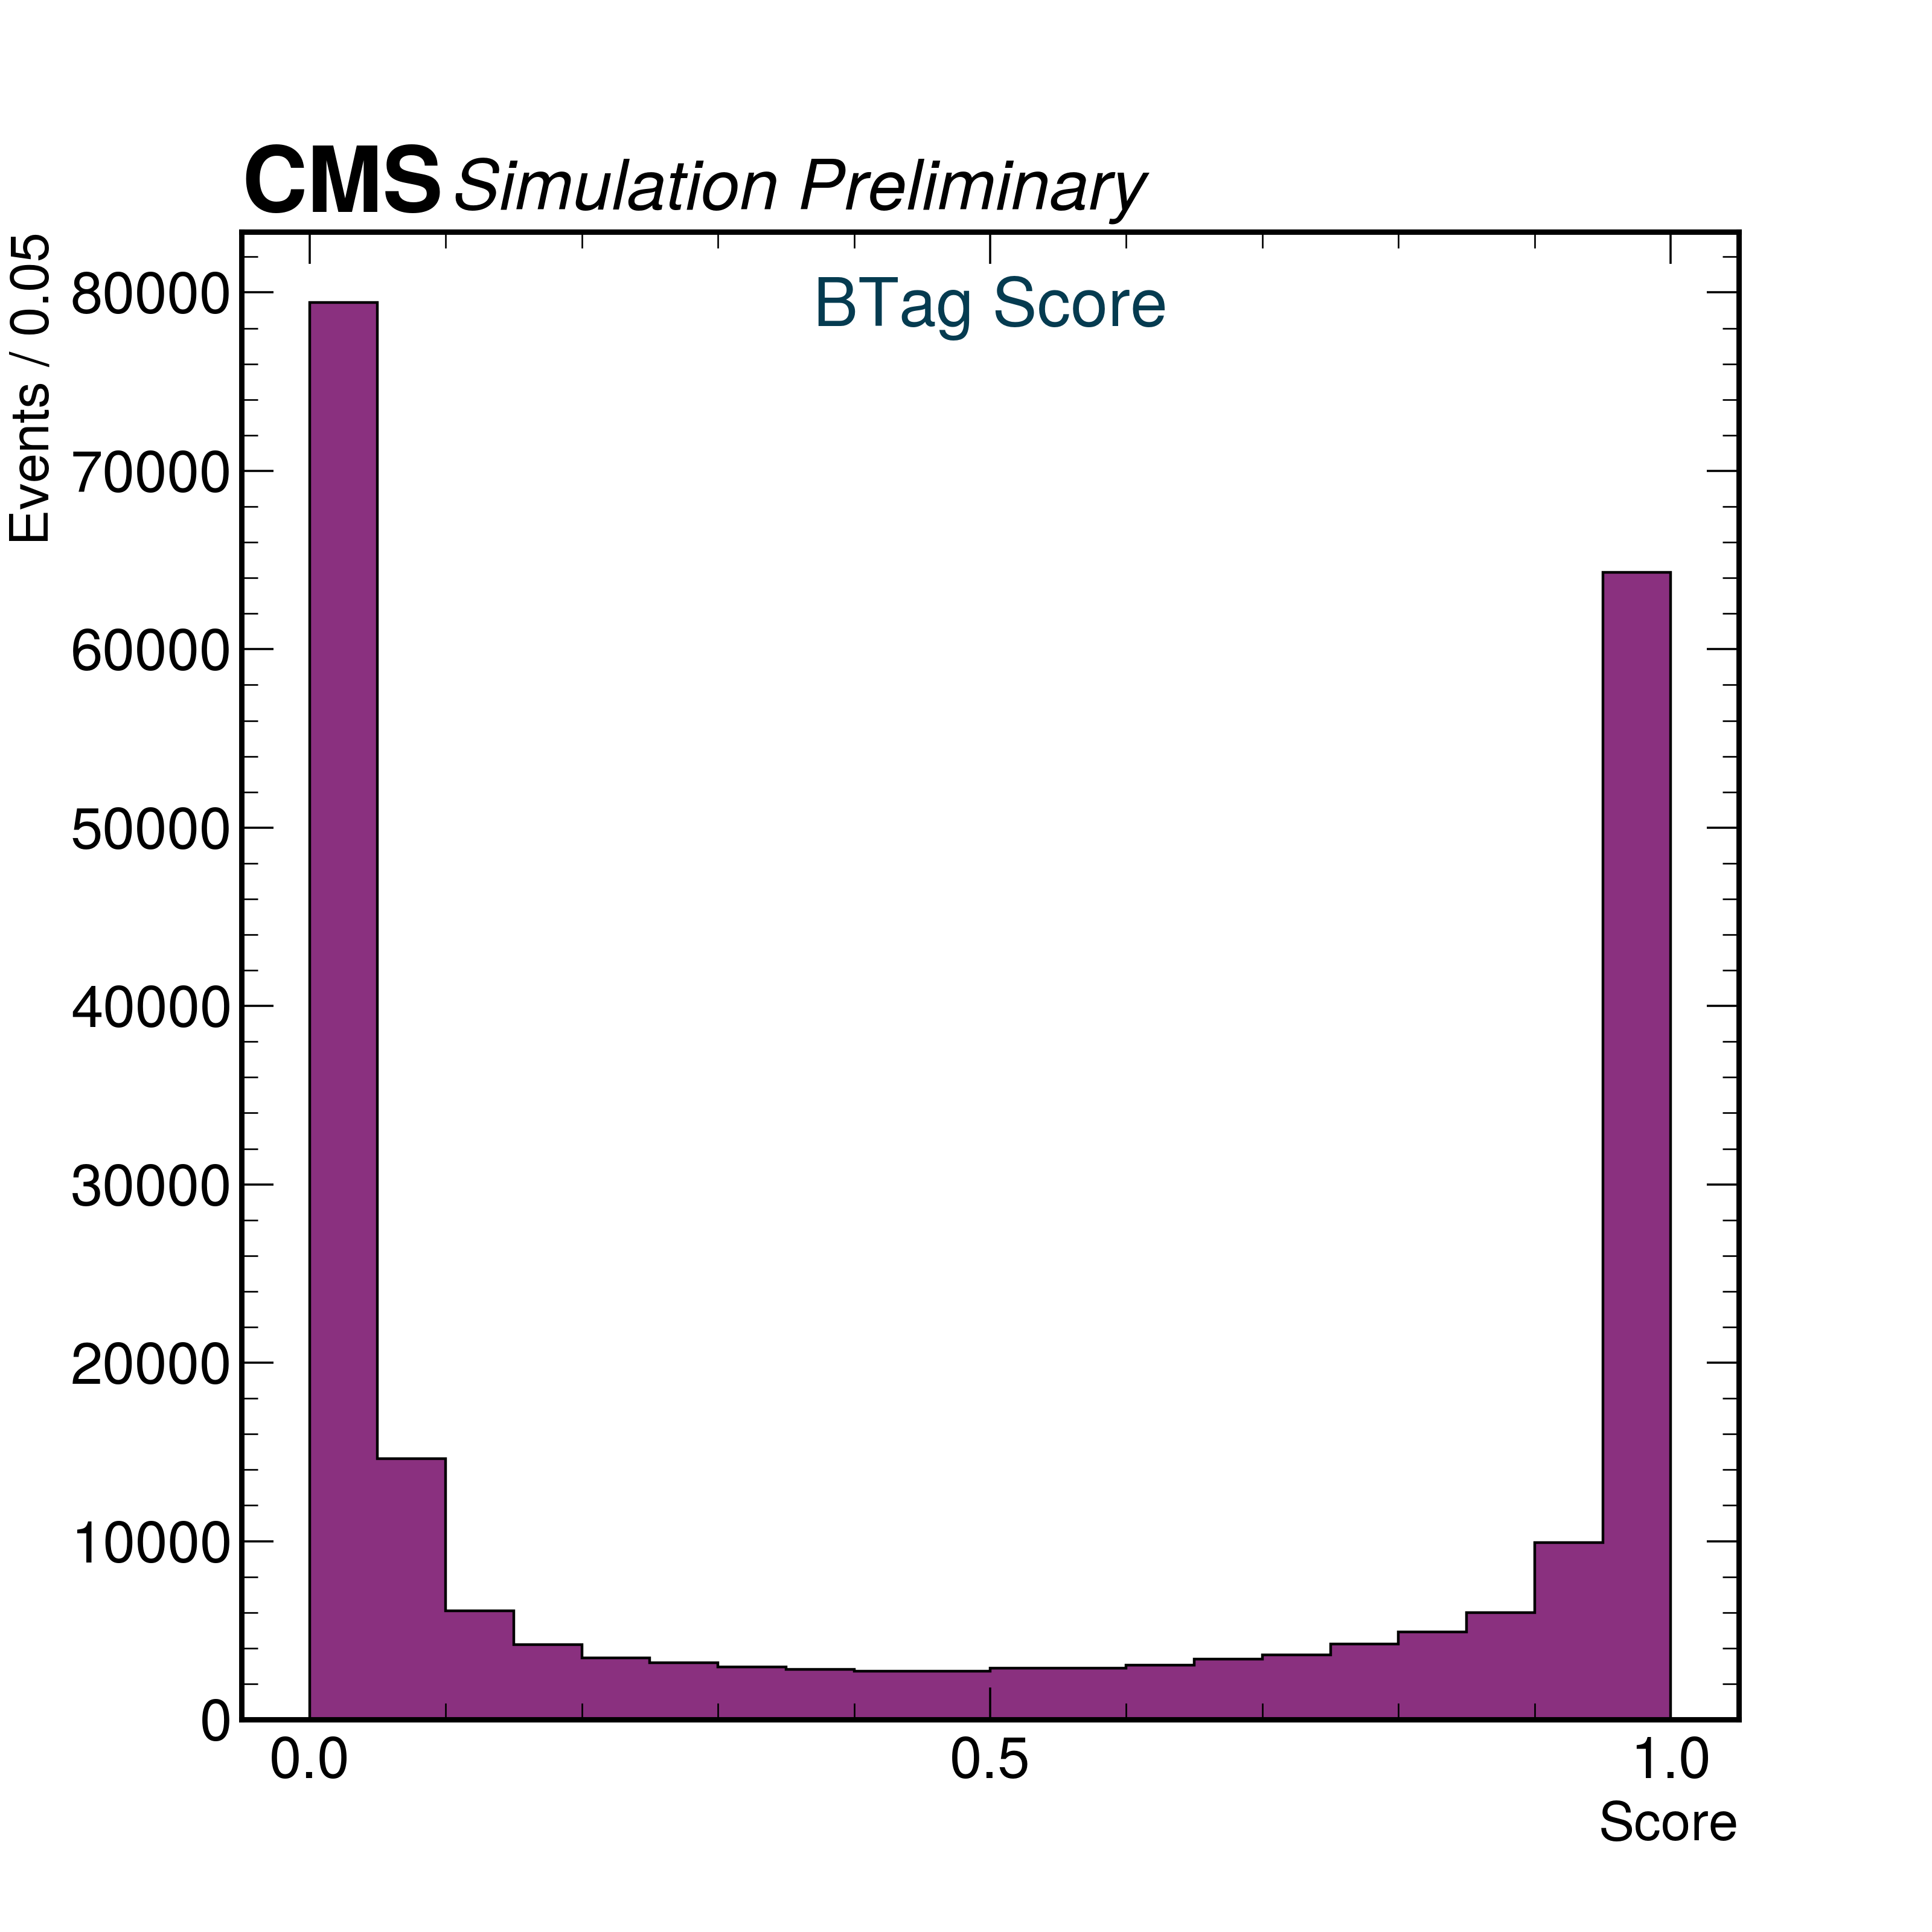
\includegraphics[width=1\textwidth]{../Archive/KinemPlots/TagMC.png }
          \label{TagMC} 
          \caption{BTag score for signal MC sample}
        \end{figure} 
        \column{0.38\textwidth} 
        \begin{itemize} 
          \raggedright 
          \small
          \item {Btagger used : \texttt{btagDeepFlavB}} 
          \item {Sample used: \texttt{MonoHTobb\_ZpBaryonic}} 
          \item Lots of bjets in Signal MC 
        \end{itemize}
      \end{columns} 
    \end{frame} 
    
    
  \begin{frame}[fragile]{BTag Scores : Data} 
    \begin{columns}
      \column{0.58\textwidth} 
      \begin{figure} 
        \centering 
        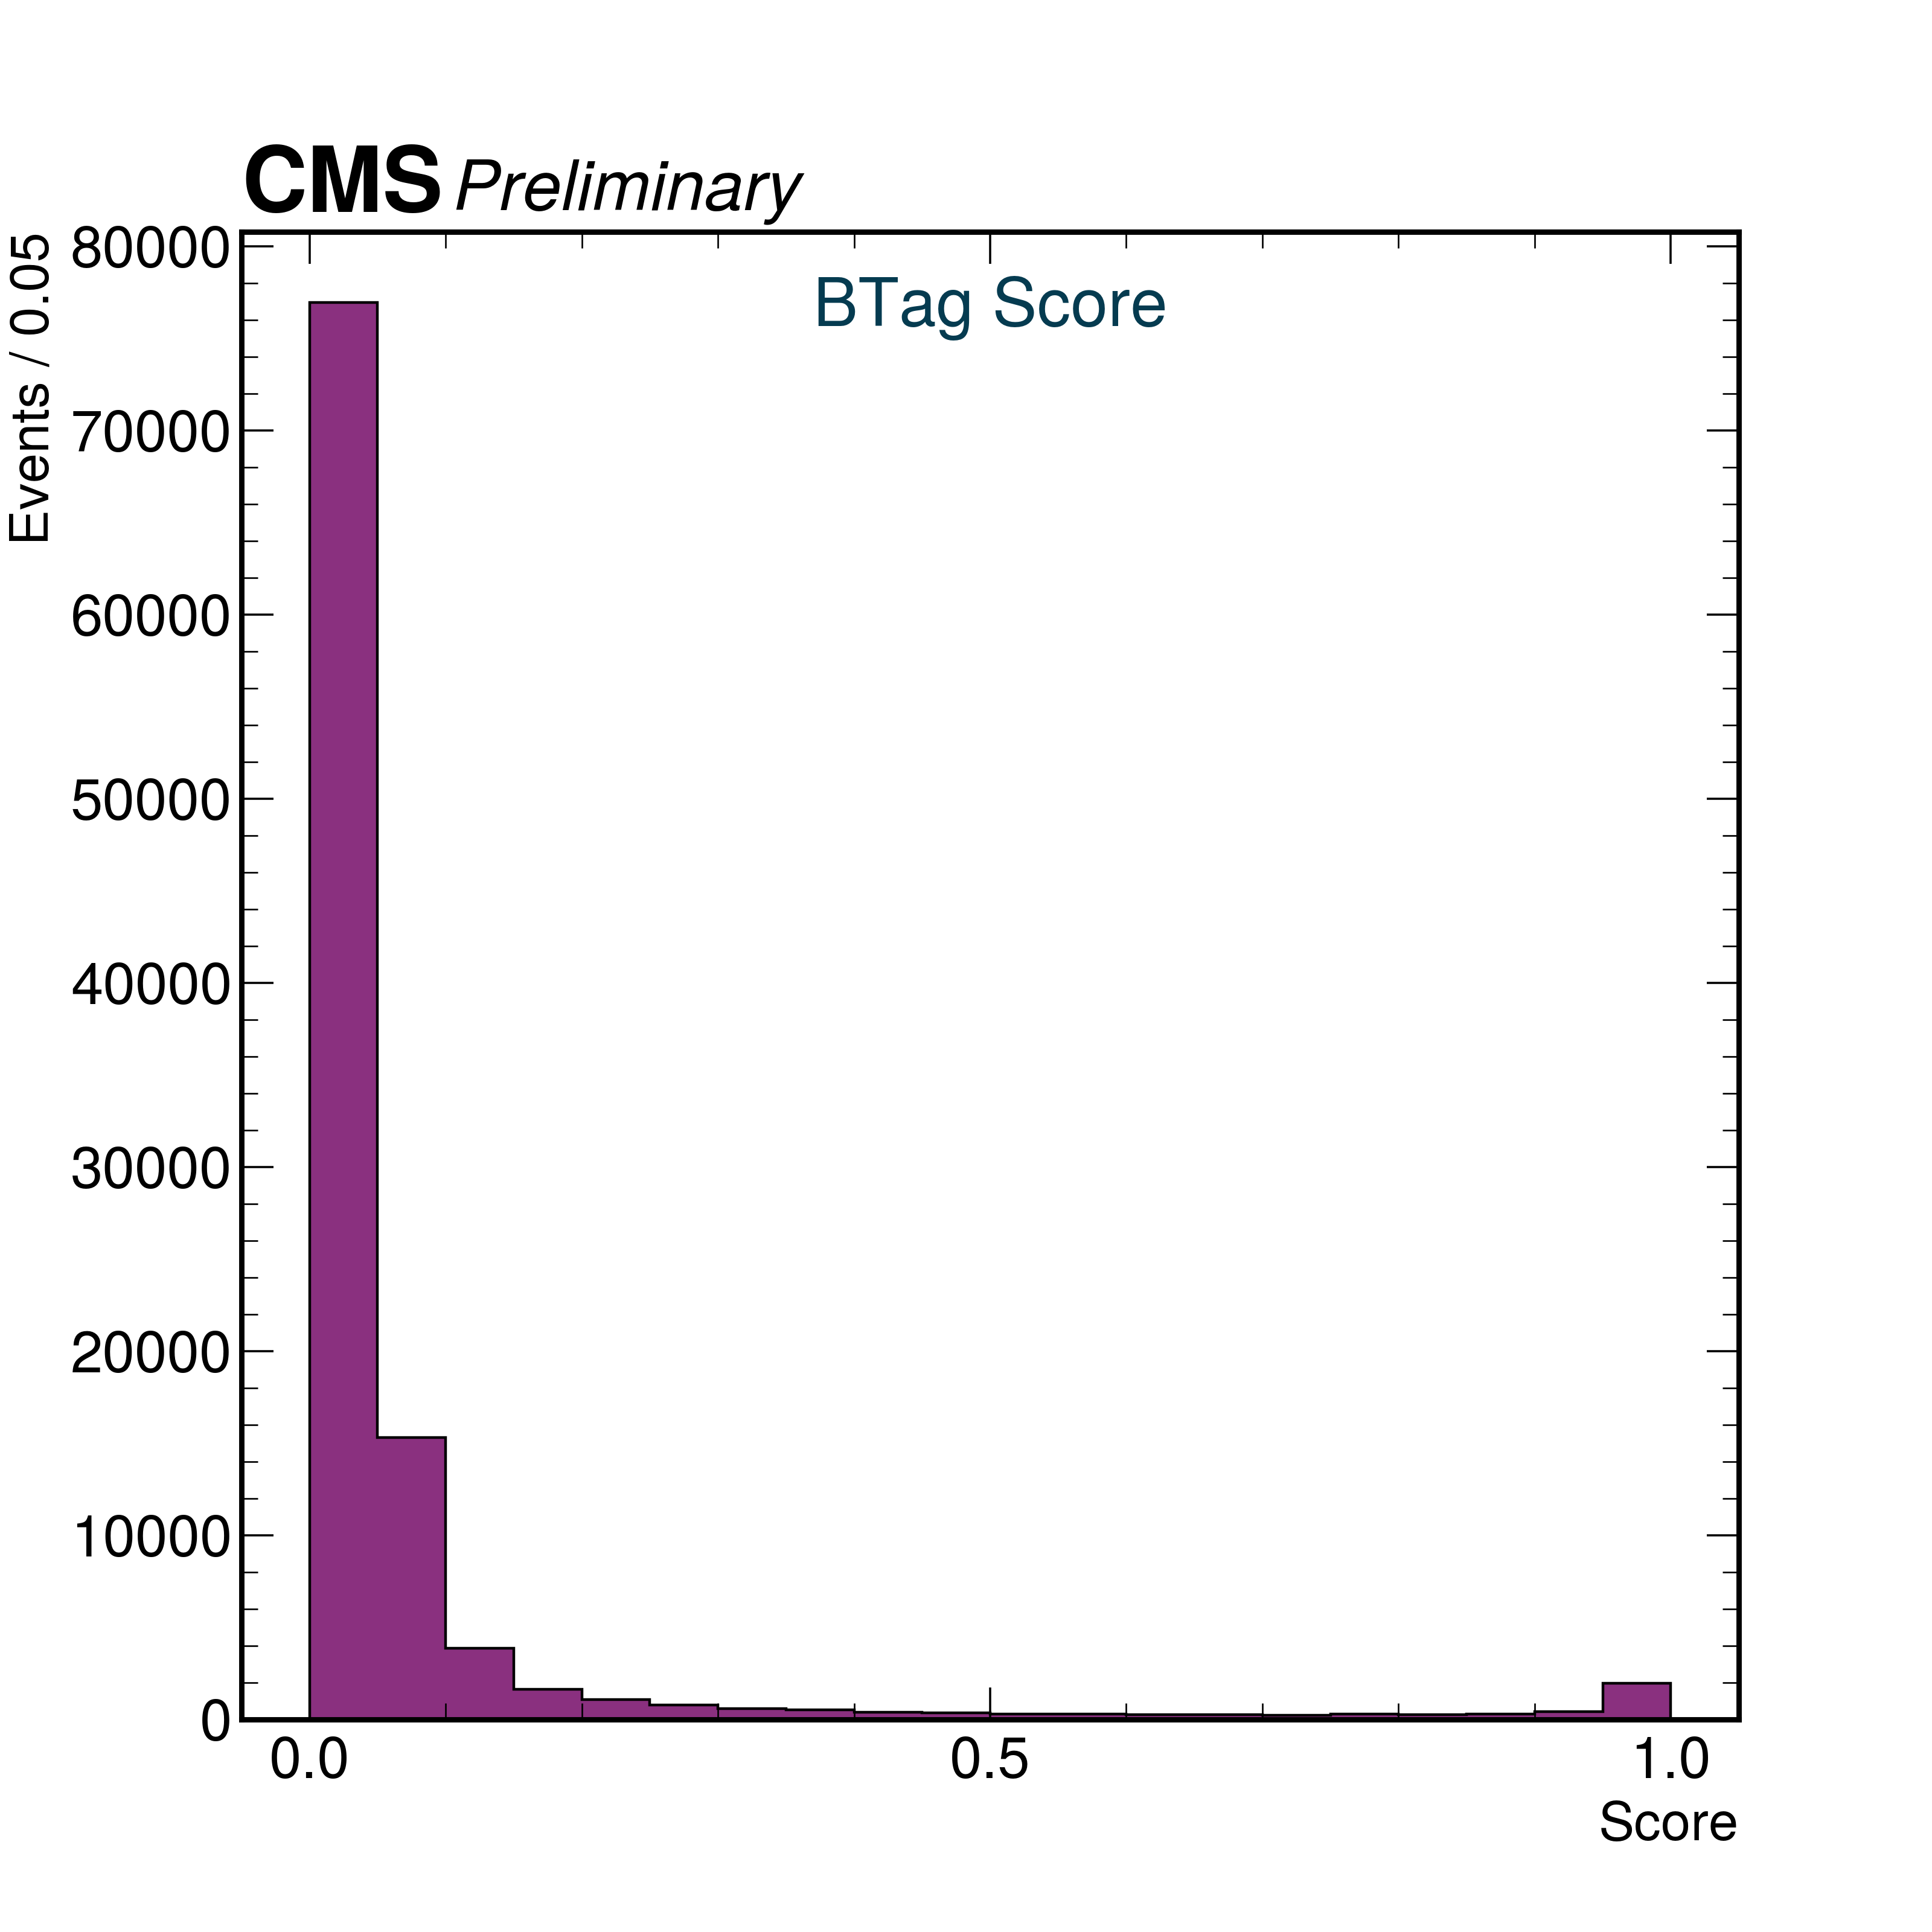
\includegraphics[width=1\textwidth]{../Archive/KinemPlots/TagData.png }
        \label{TagData} 
        \caption{BTag score for Data samples}
      \end{figure} 
      \column{0.38\textwidth} 
      \begin{itemize} 
        \raggedright 
        \small
        \item {Btagger used : \texttt{btagDeepFlavB}} 
        \item {Sample used: \texttt{Run2018A/MET}} 
        \item Less number of bjets in Data
      \end{itemize}
    \end{columns} 
  \end{frame} 
    
    
   \begin{frame}[fragile]{Jet $p_t$ : MC} 
    \begin{columns}
    \column{0.58\textwidth} 
    \begin{figure} 
    \centering 
     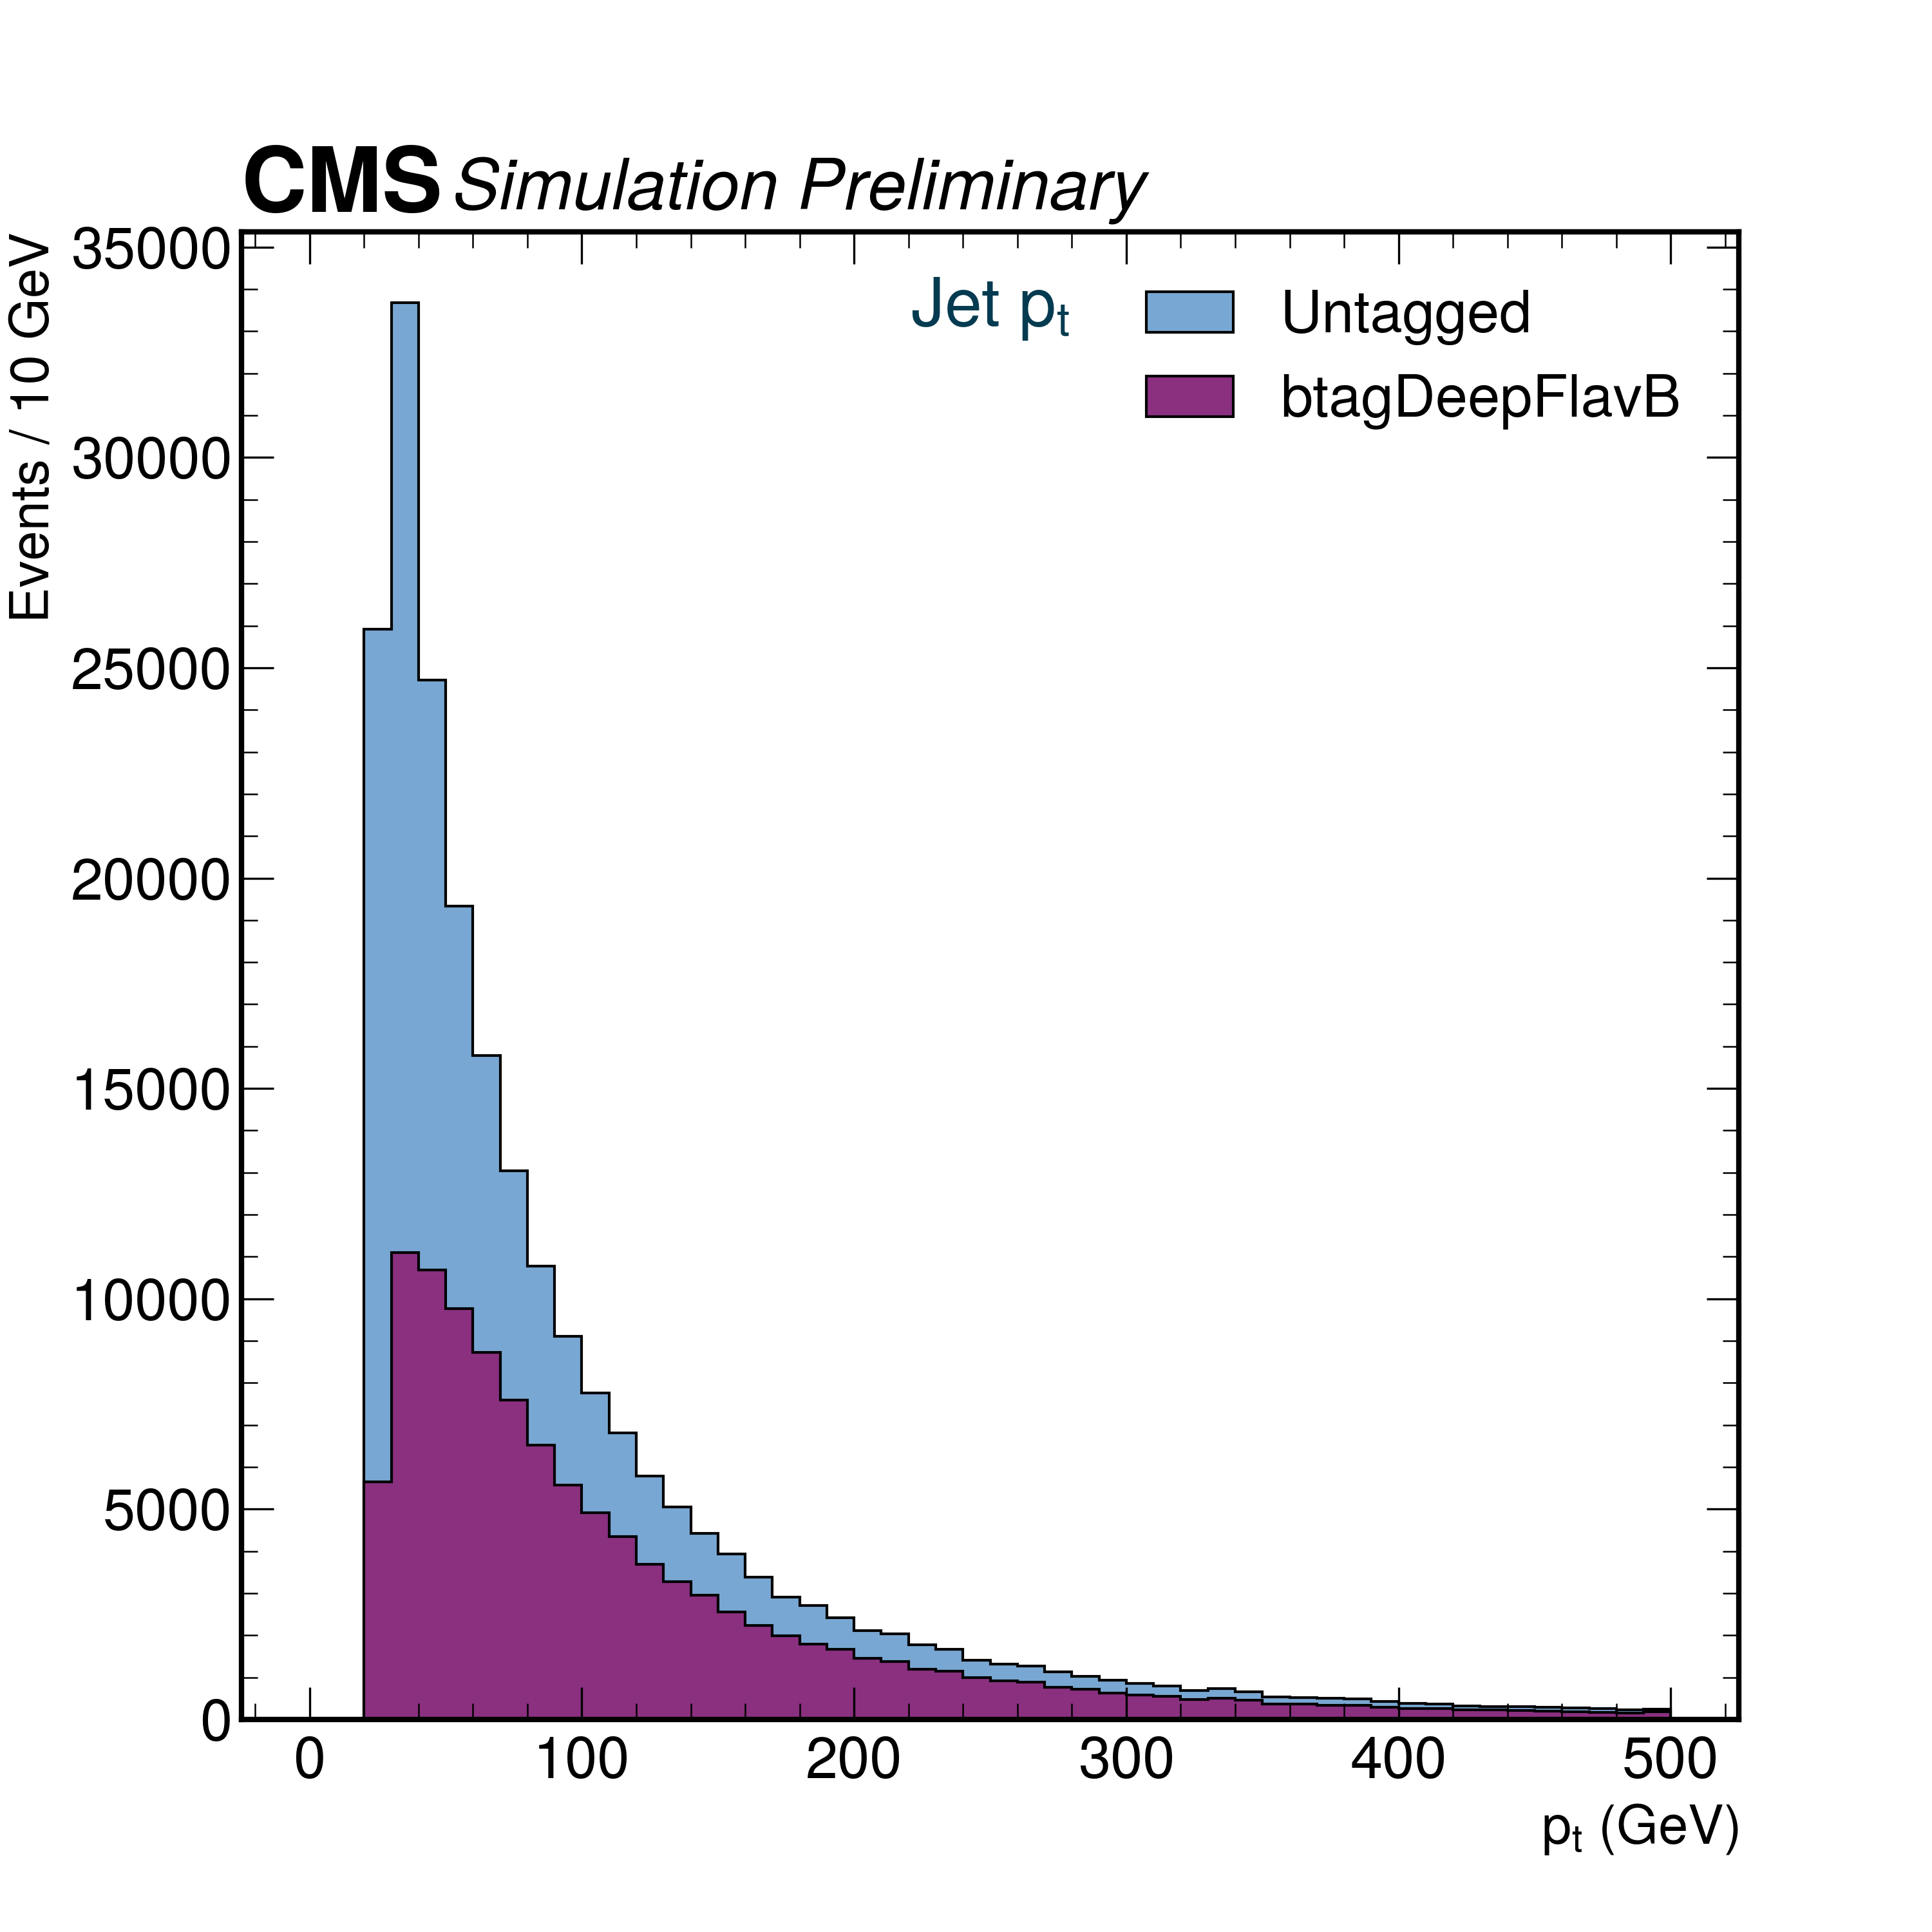
\includegraphics[width=1\textwidth]{../Archive/KinemPlots/JetsMC.png }
    \label{JetMC} 
    \caption{Jet $p_t$ of signal MC samples}
    \end{figure} 
    \column{0.38\textwidth} 
    \begin{itemize} 
    \raggedright 
    \small
    \item Basic selections : $p_t > 25 GeV $ and $|\eta | < 2.5 $
    \item {Btagger used : \texttt{btagDeepFlavB}} 
    \item {Sample used: \texttt{MonoHTobb\_ZpBaryonic}} 
    \item Medium Weight Parameter used for ak4bjets : 0.3040  
    \end{itemize}
    \end{columns} 
    \end{frame} 
    
    
   \begin{frame}[fragile]{Jet $p_t$ : Data} 
    \begin{columns}
    \column{0.58\textwidth} 
    \begin{figure} 
    \centering 
     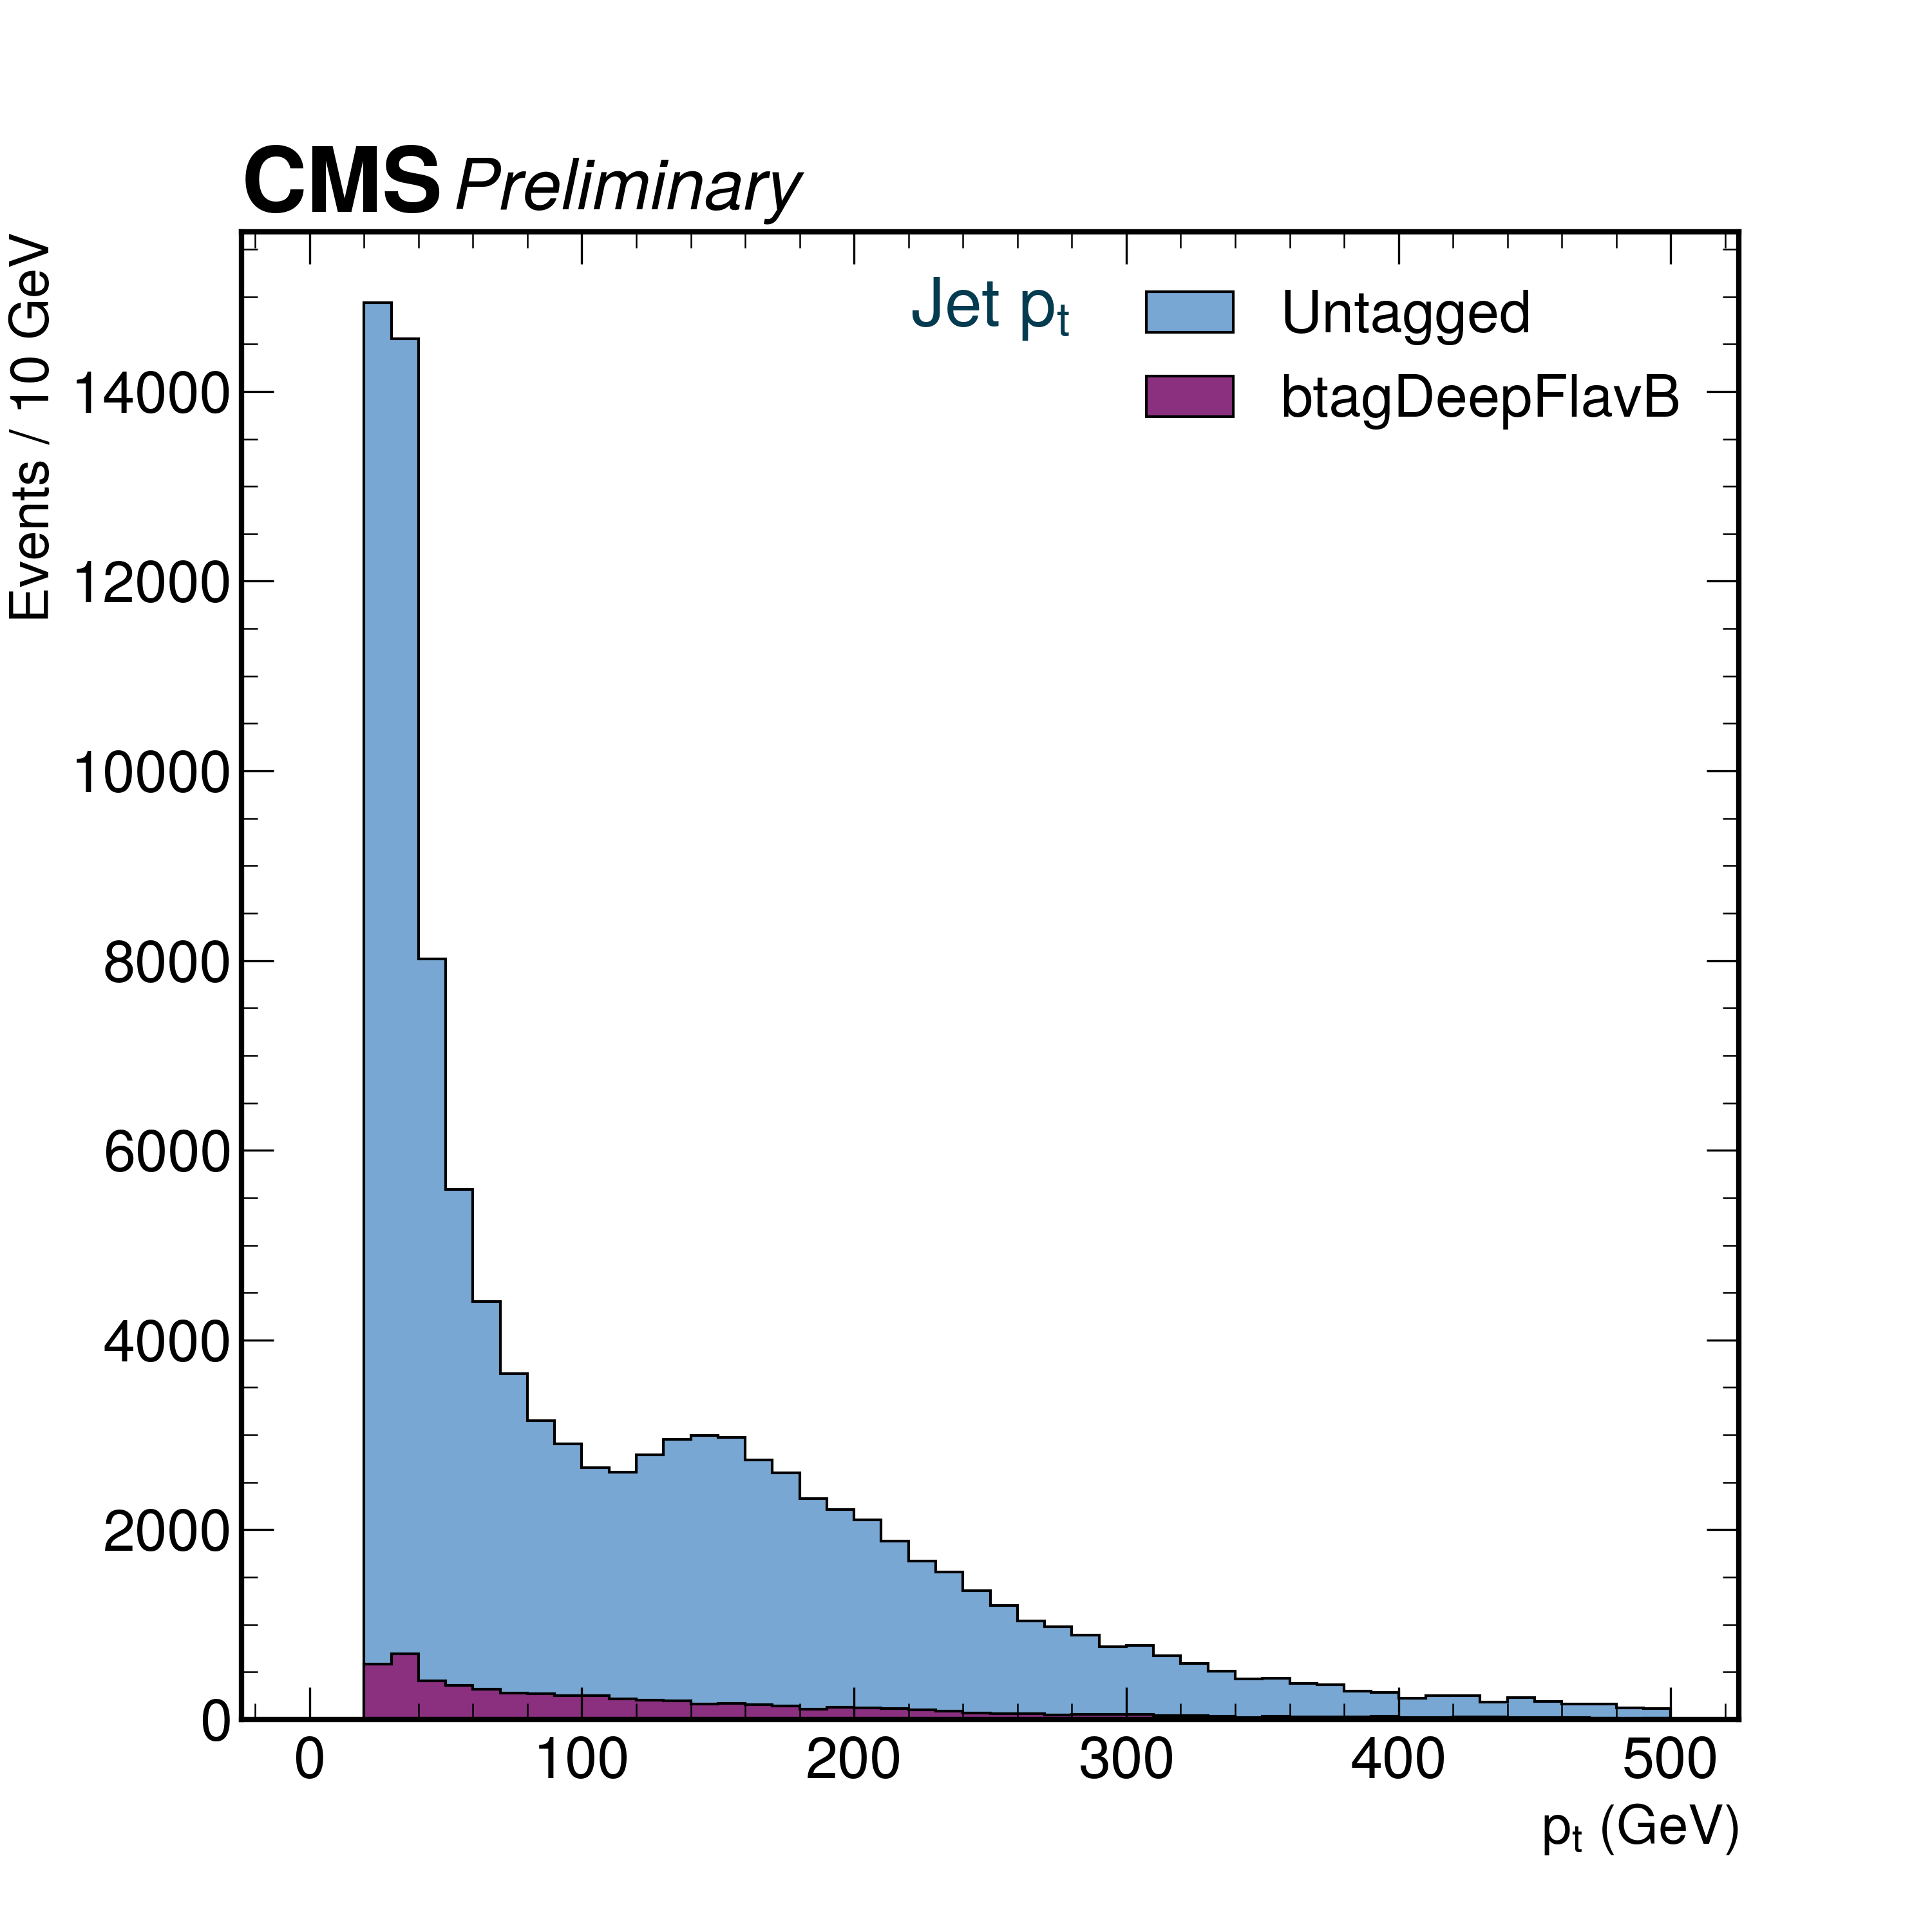
\includegraphics[width=1\textwidth]{../Archive/KinemPlots/JetsData.png }
    \label{JetData} 
    \caption{Jet $p_t$ of Data samples}
    \end{figure} 
    \column{0.38\textwidth} 
    \begin{itemize} 
    \raggedright 
    \small
    \item Basic selections : $p_t > 25 GeV $ and $|\eta | < 2.5 $
    \item {Btagger used : \texttt{btagDeepFlavB}} 
    \item {Sample used: \texttt{Run2018A/MET}} 
    \item Medium Weight Parameter used for ak4bjets : 0.3040
    \item Not as predictable as signal MC 
    \end{itemize}
    \end{columns} 
    \end{frame} 
    
    
   \begin{frame}[fragile]{DiJet mass : MC} 
    \begin{columns}
    \column{0.58\textwidth} 
    \begin{figure} 
    \centering 
     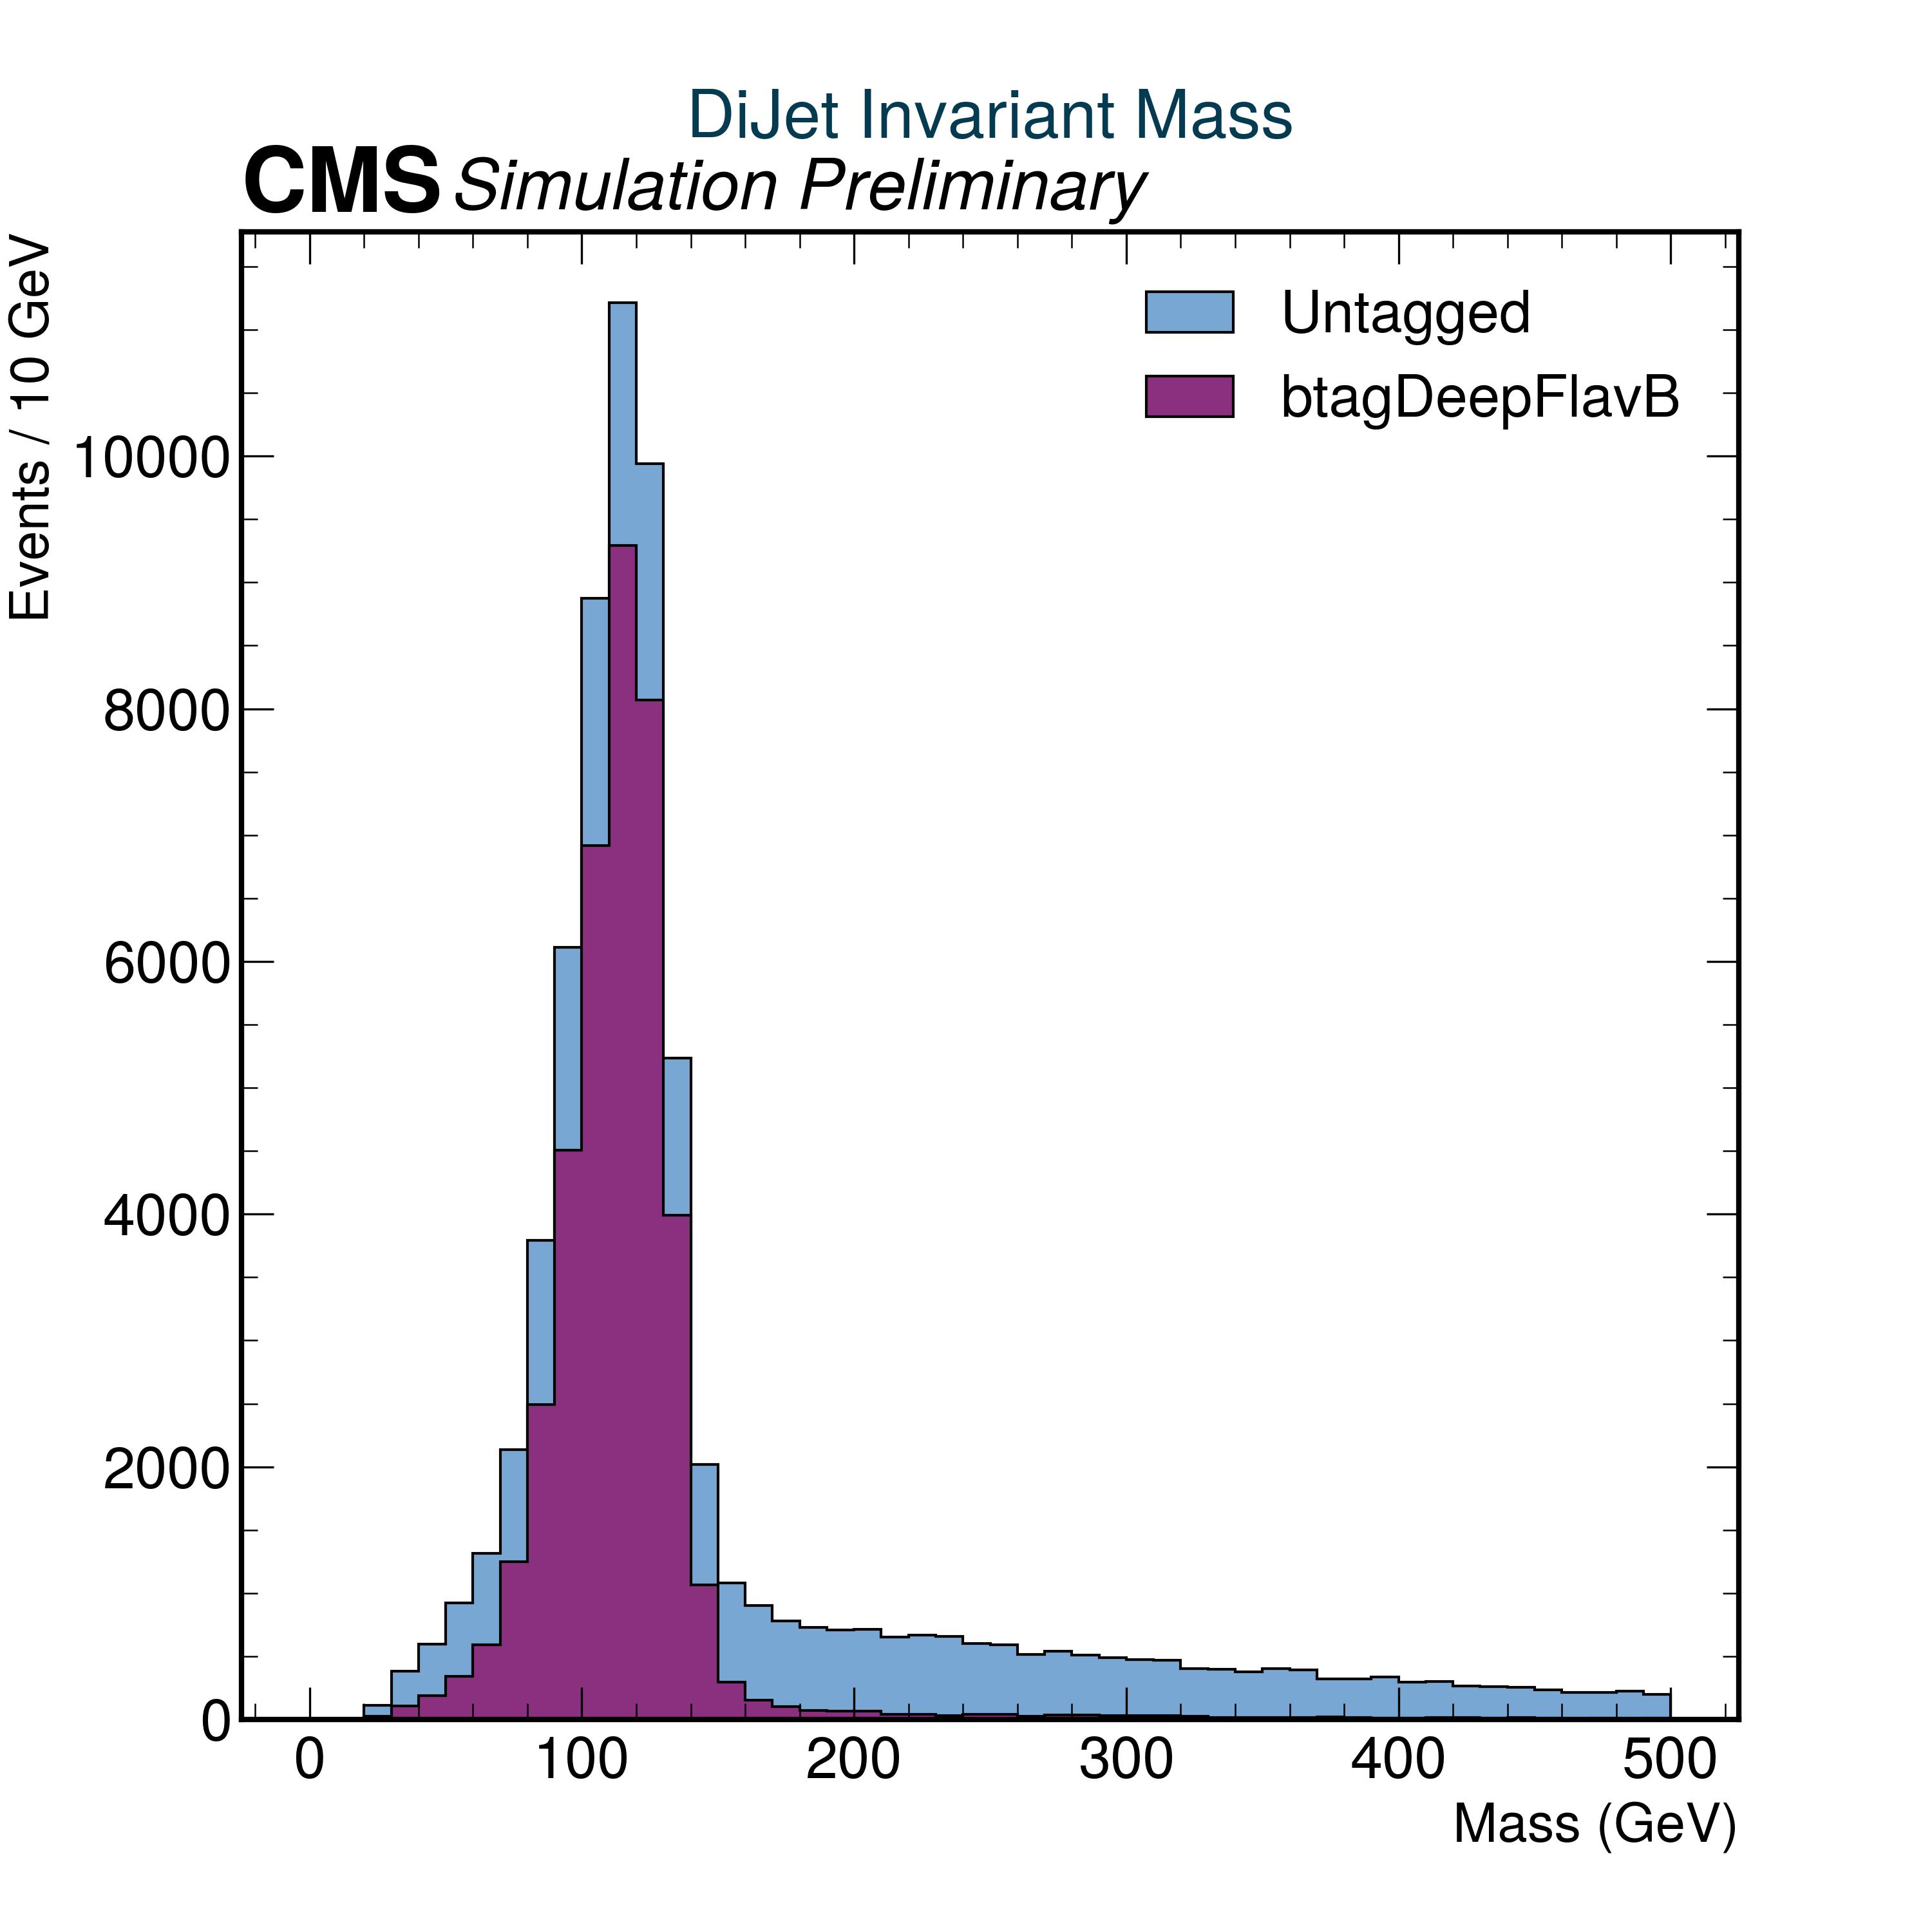
\includegraphics[width=1\textwidth]{../Archive/KinemPlots/DiJetsMC.png }
    \label{DiJetMC} 
    \caption{DiJet mass of signal MC samples}
    \end{figure} 
    \column{0.38\textwidth} 
    \begin{itemize} 
    \raggedright 
    \small
    \item Basic selections : $p_t > 25 GeV $ and $|\eta | < 2.5 $ for each jet
    \item {Btagger used : \texttt{btagDeepFlavB}} 
    \item {Sample used: \texttt{MonoHTobb\_ZpBaryonic}} 
    \item Medium Weight Parameter used for ak4bjets selection : 0.3040
    \item Peaks around SM Higgs mass 
    \end{itemize}
    \end{columns} 
    \end{frame} 
    
    
   \begin{frame}[fragile]{DiJet mass : Data} 
    \begin{columns}
    \column{0.58\textwidth} 
    \begin{figure} 
    \centering 
     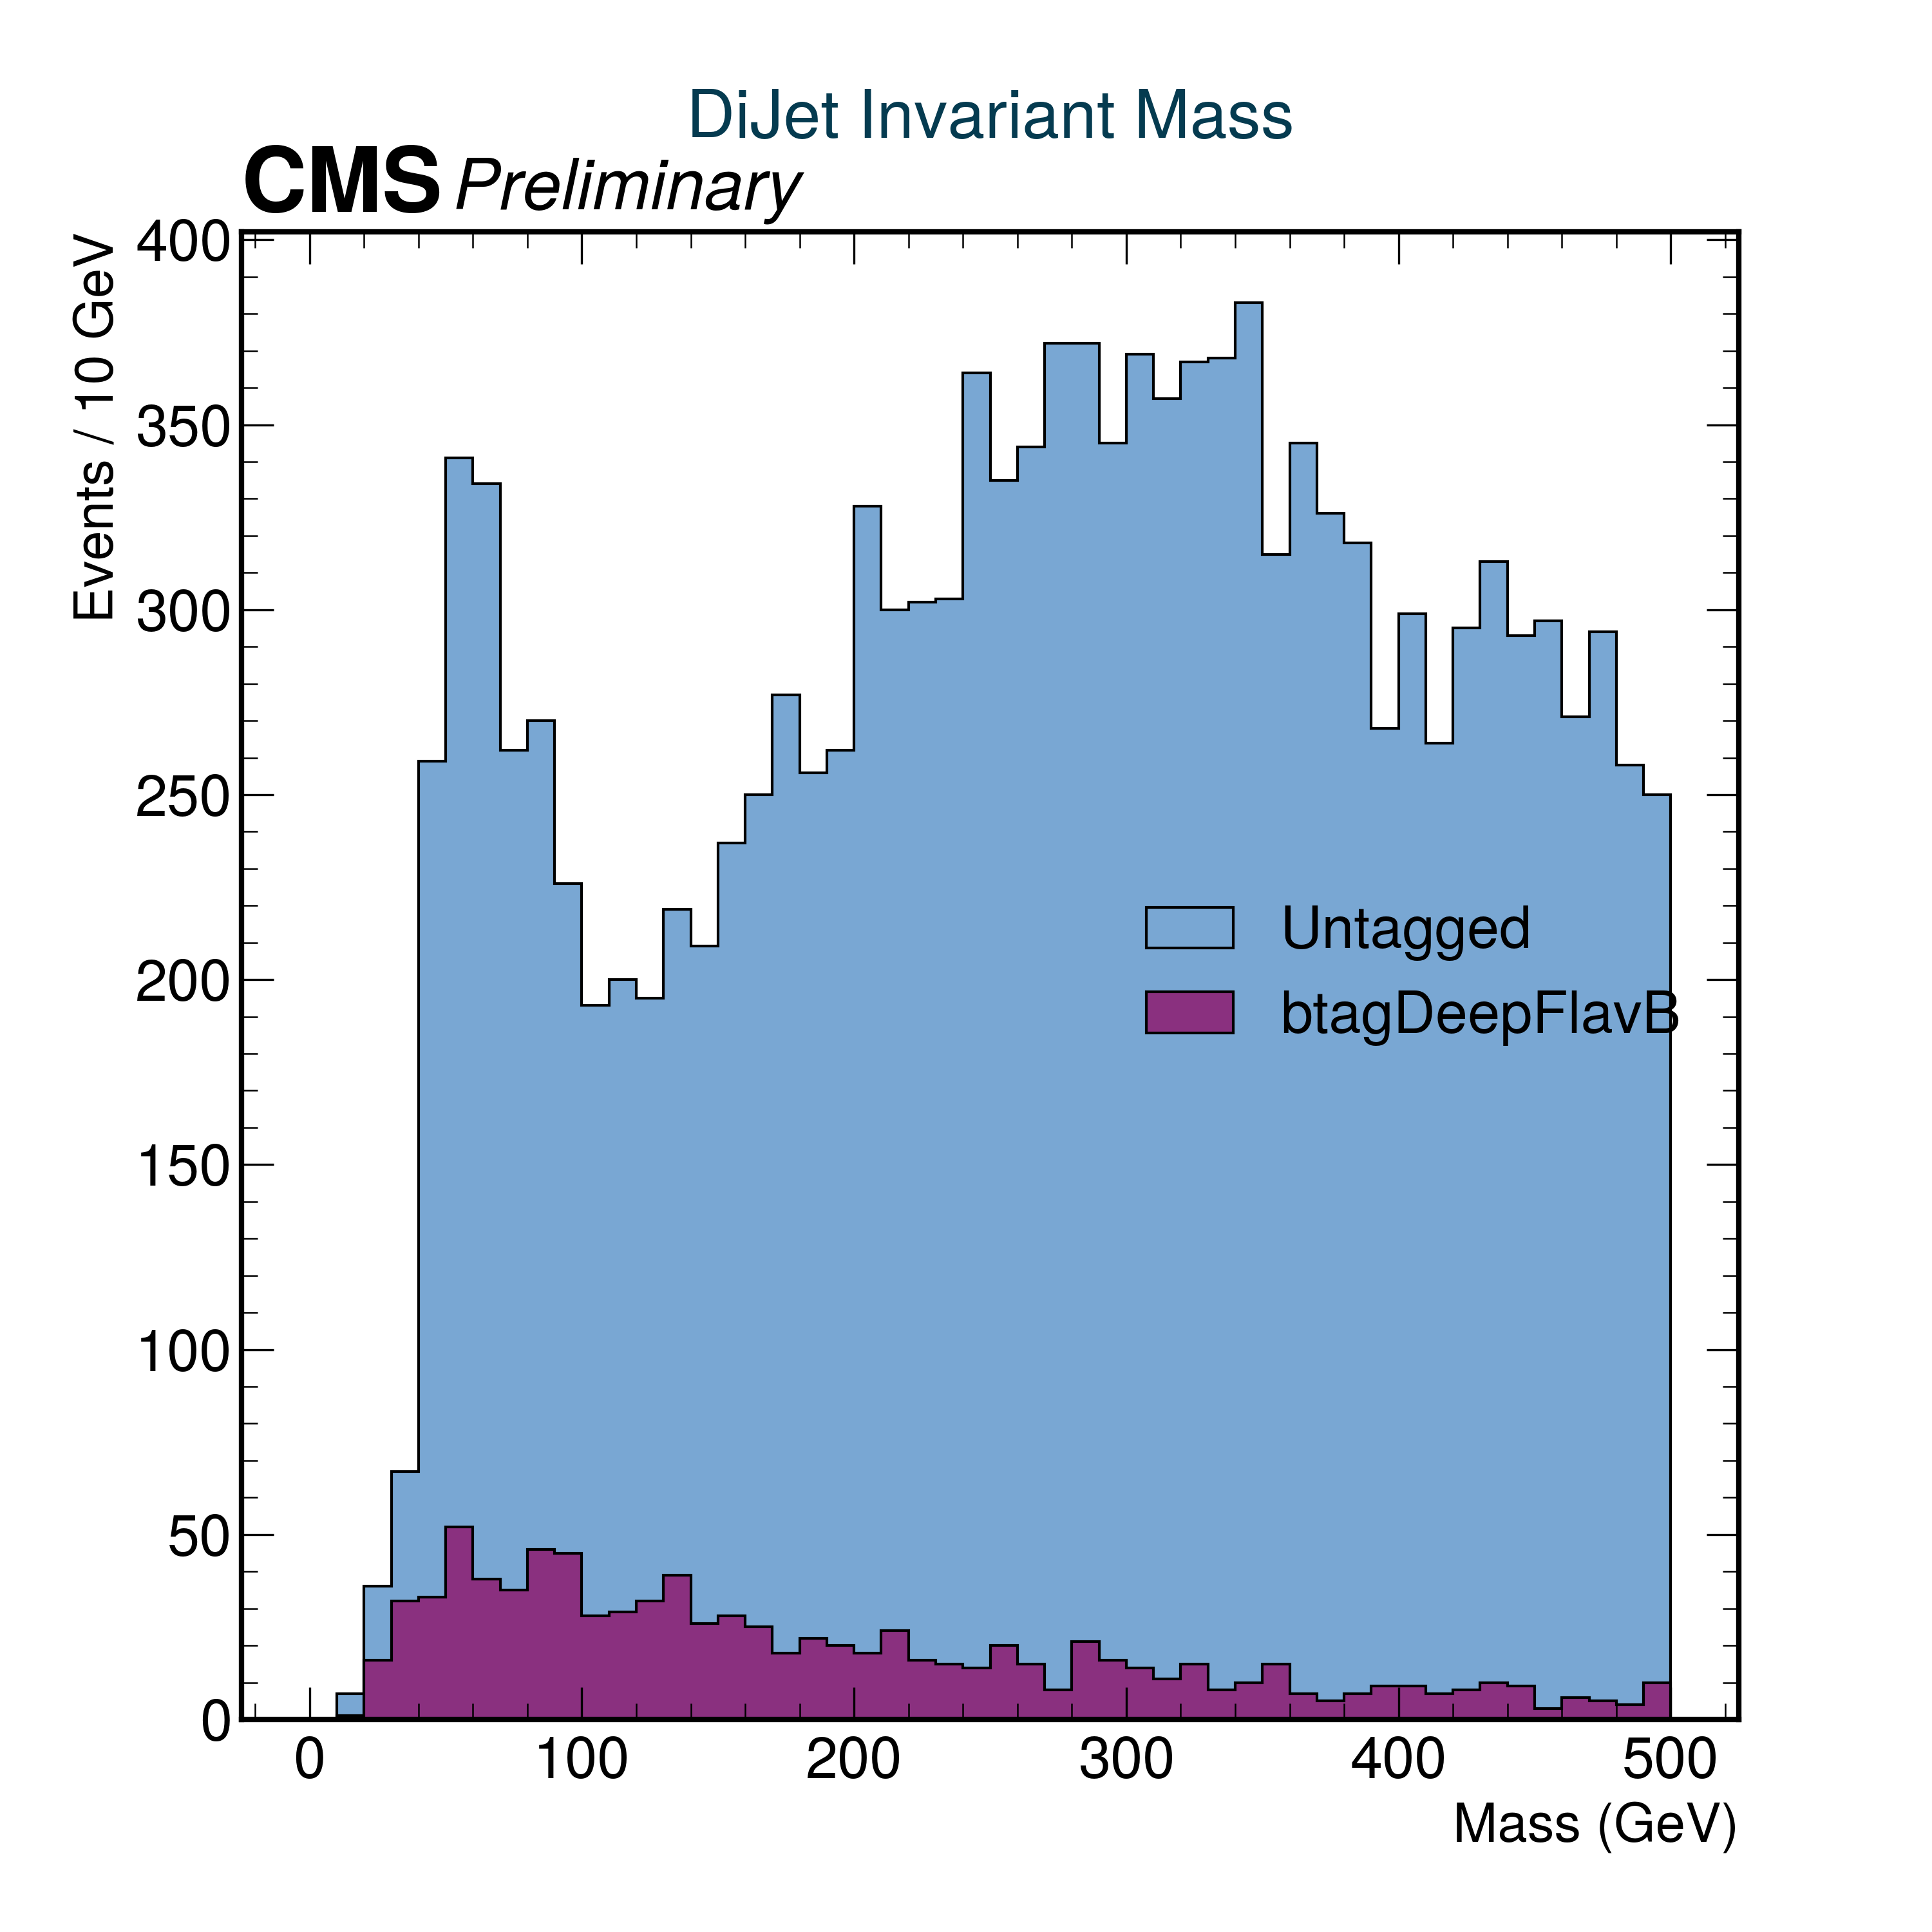
\includegraphics[width=1\textwidth]{../Archive/KinemPlots/DiJetsData.png }
    \label{DiJetData} 
    \caption{DiJet mass of Data samples}
    \end{figure} 
    \column{0.38\textwidth} 
    \begin{itemize} 
    \raggedright 
    \small
    \item Basic selections : $p_t > 25 GeV $ and $|\eta | < 2.5 $ for each jet
    \item {Btagger used : \texttt{btagDeepFlavB}} 
    \item {Sample used: \texttt{Run2018A/MET}} 
    \item Medium Weight Parameter used for ak4bjets selection : 0.3040
    \item Lot of noise, no clear structure 
    \end{itemize}
    \end{columns} 
    \end{frame} 
    
    
   \begin{frame}[fragile]{MET $p_t$ : MC} 
    \begin{columns}
    \column{0.58\textwidth} 
    \begin{figure} 
    \centering 
     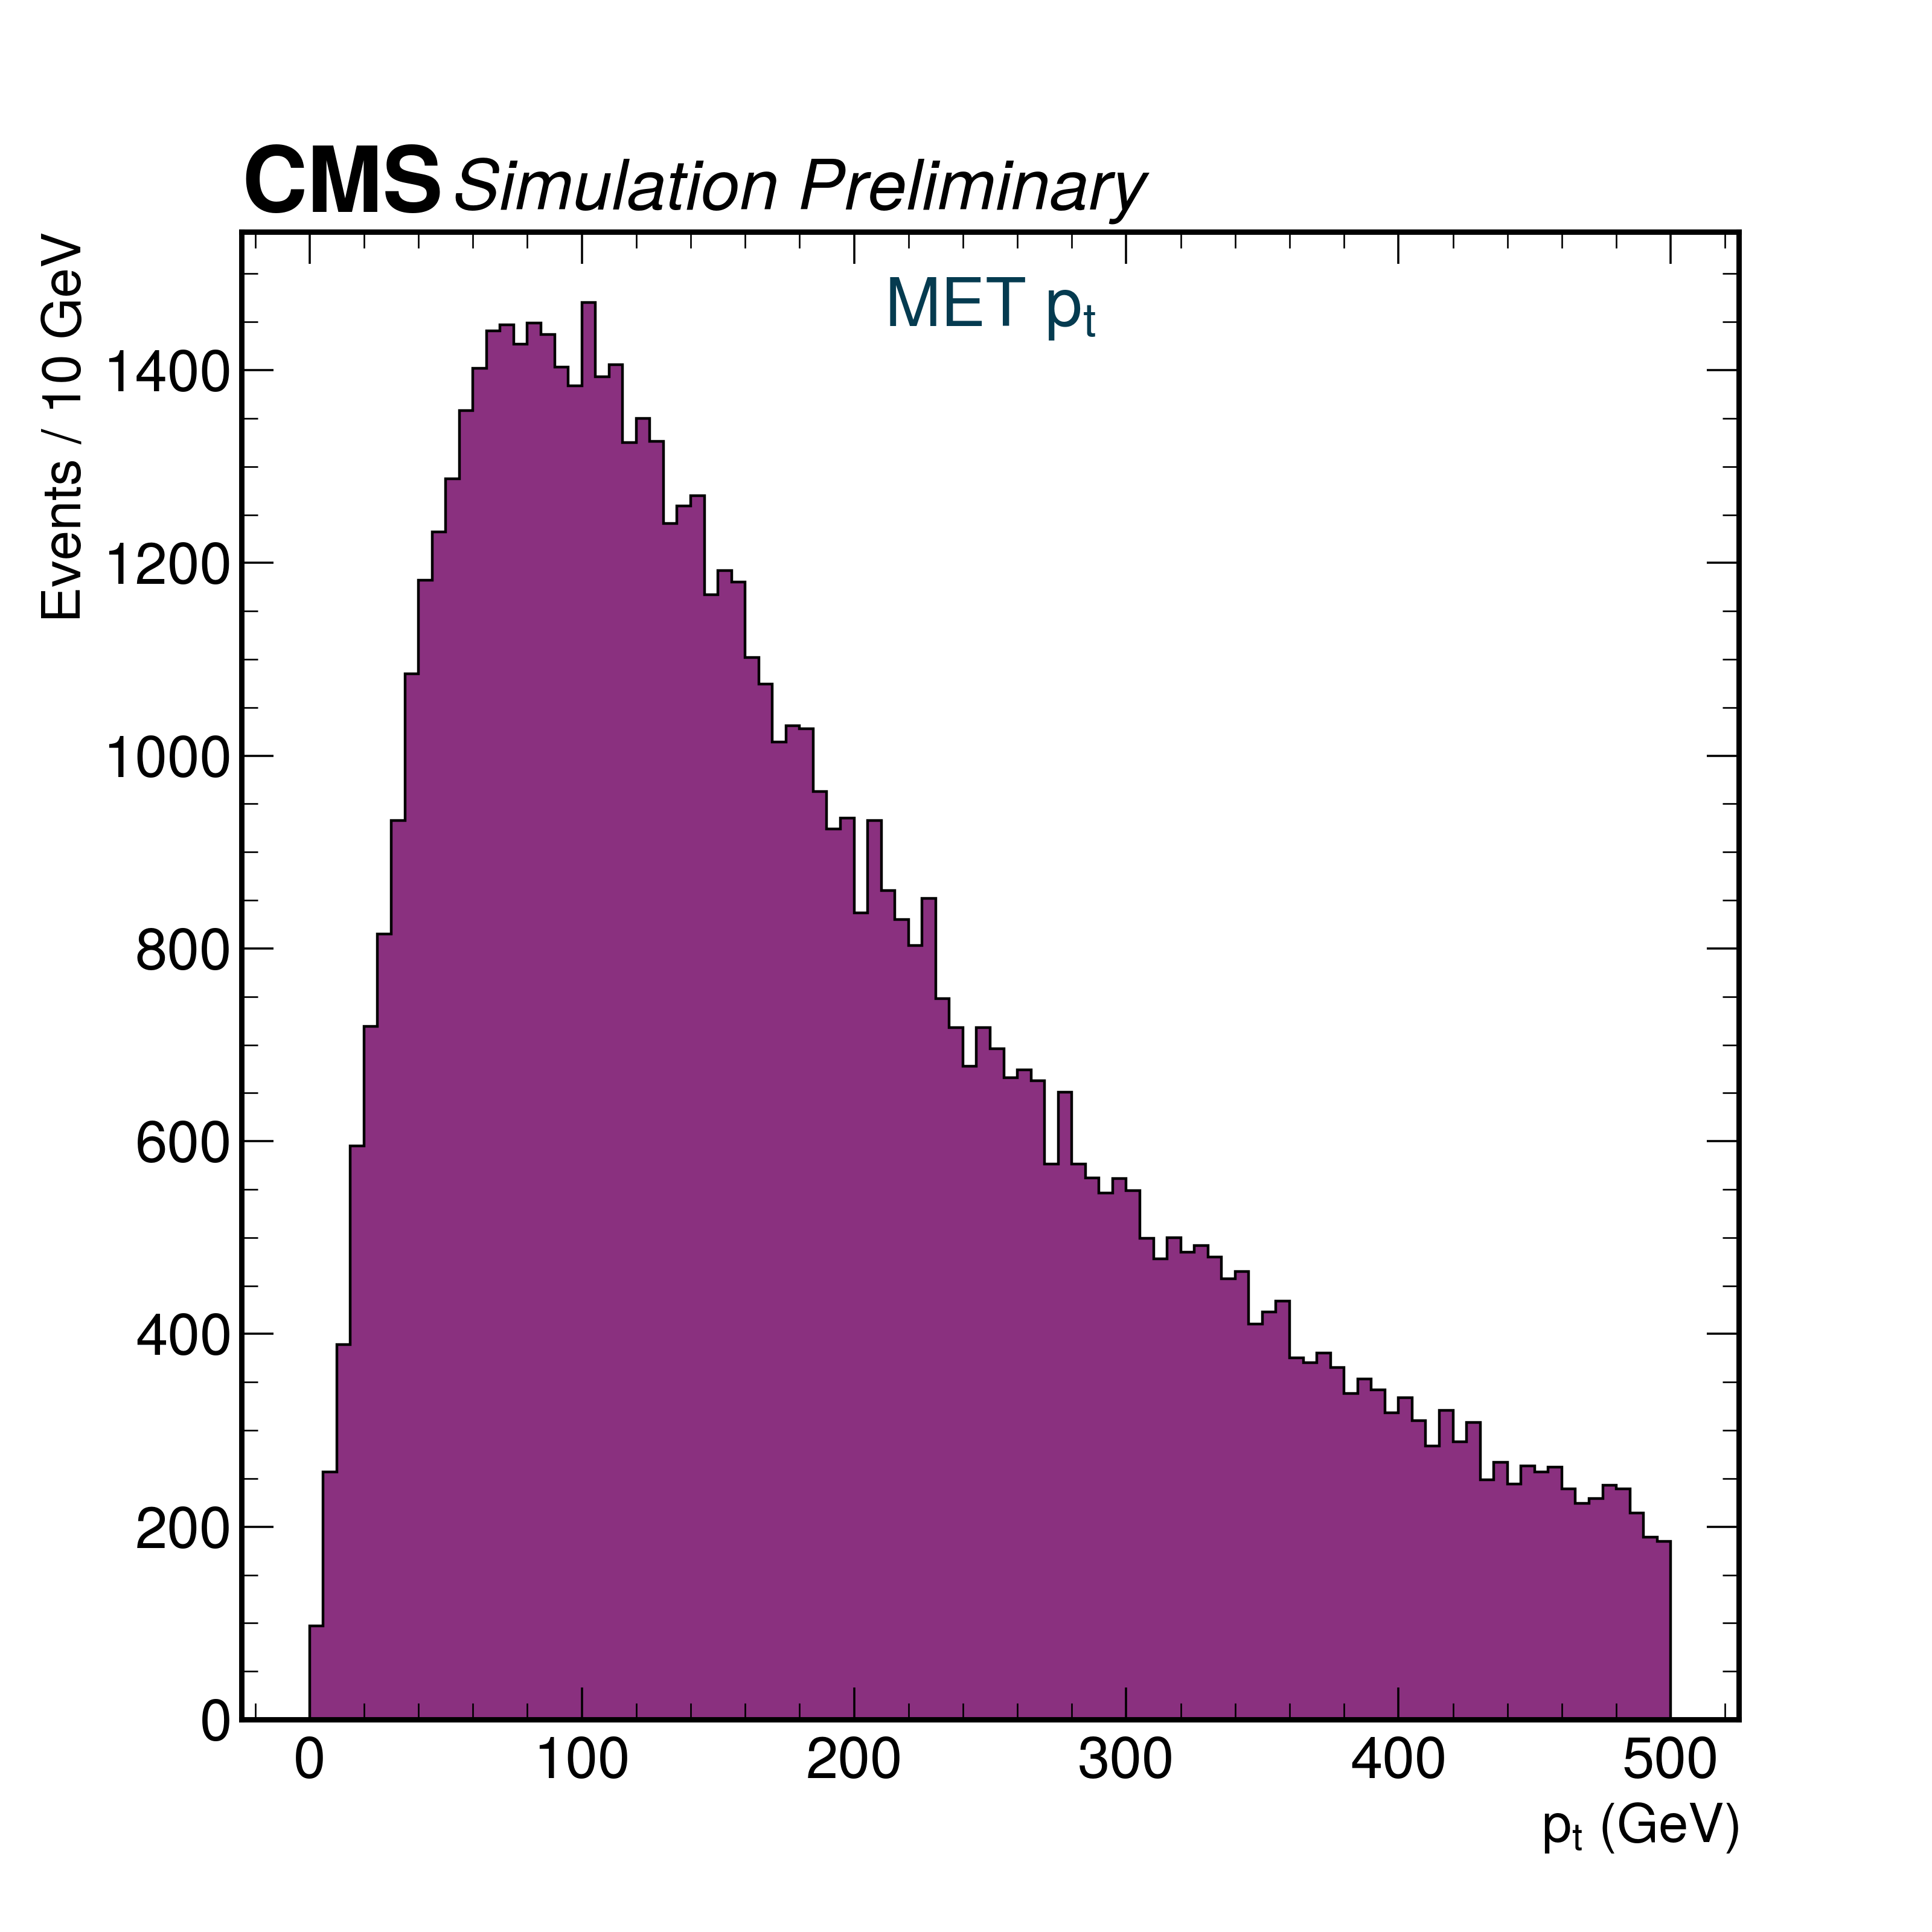
\includegraphics[width=1\textwidth]{../Archive/KinemPlots/METMC.png }
    \label{METMC} 
    \caption{MET $p_t$ for signal MC samples}
    \end{figure} 
    \column{0.38\textwidth} 
    \begin{itemize} 
    \raggedright 
    \small
    \item No filters or Trigger applied
    \end{itemize}
    \end{columns} 
    \end{frame} 
    
    
   \begin{frame}[fragile]{MET $p_t$ : Data} 
    \begin{columns}
    \column{0.58\textwidth} 
    \begin{figure} 
    \centering 
     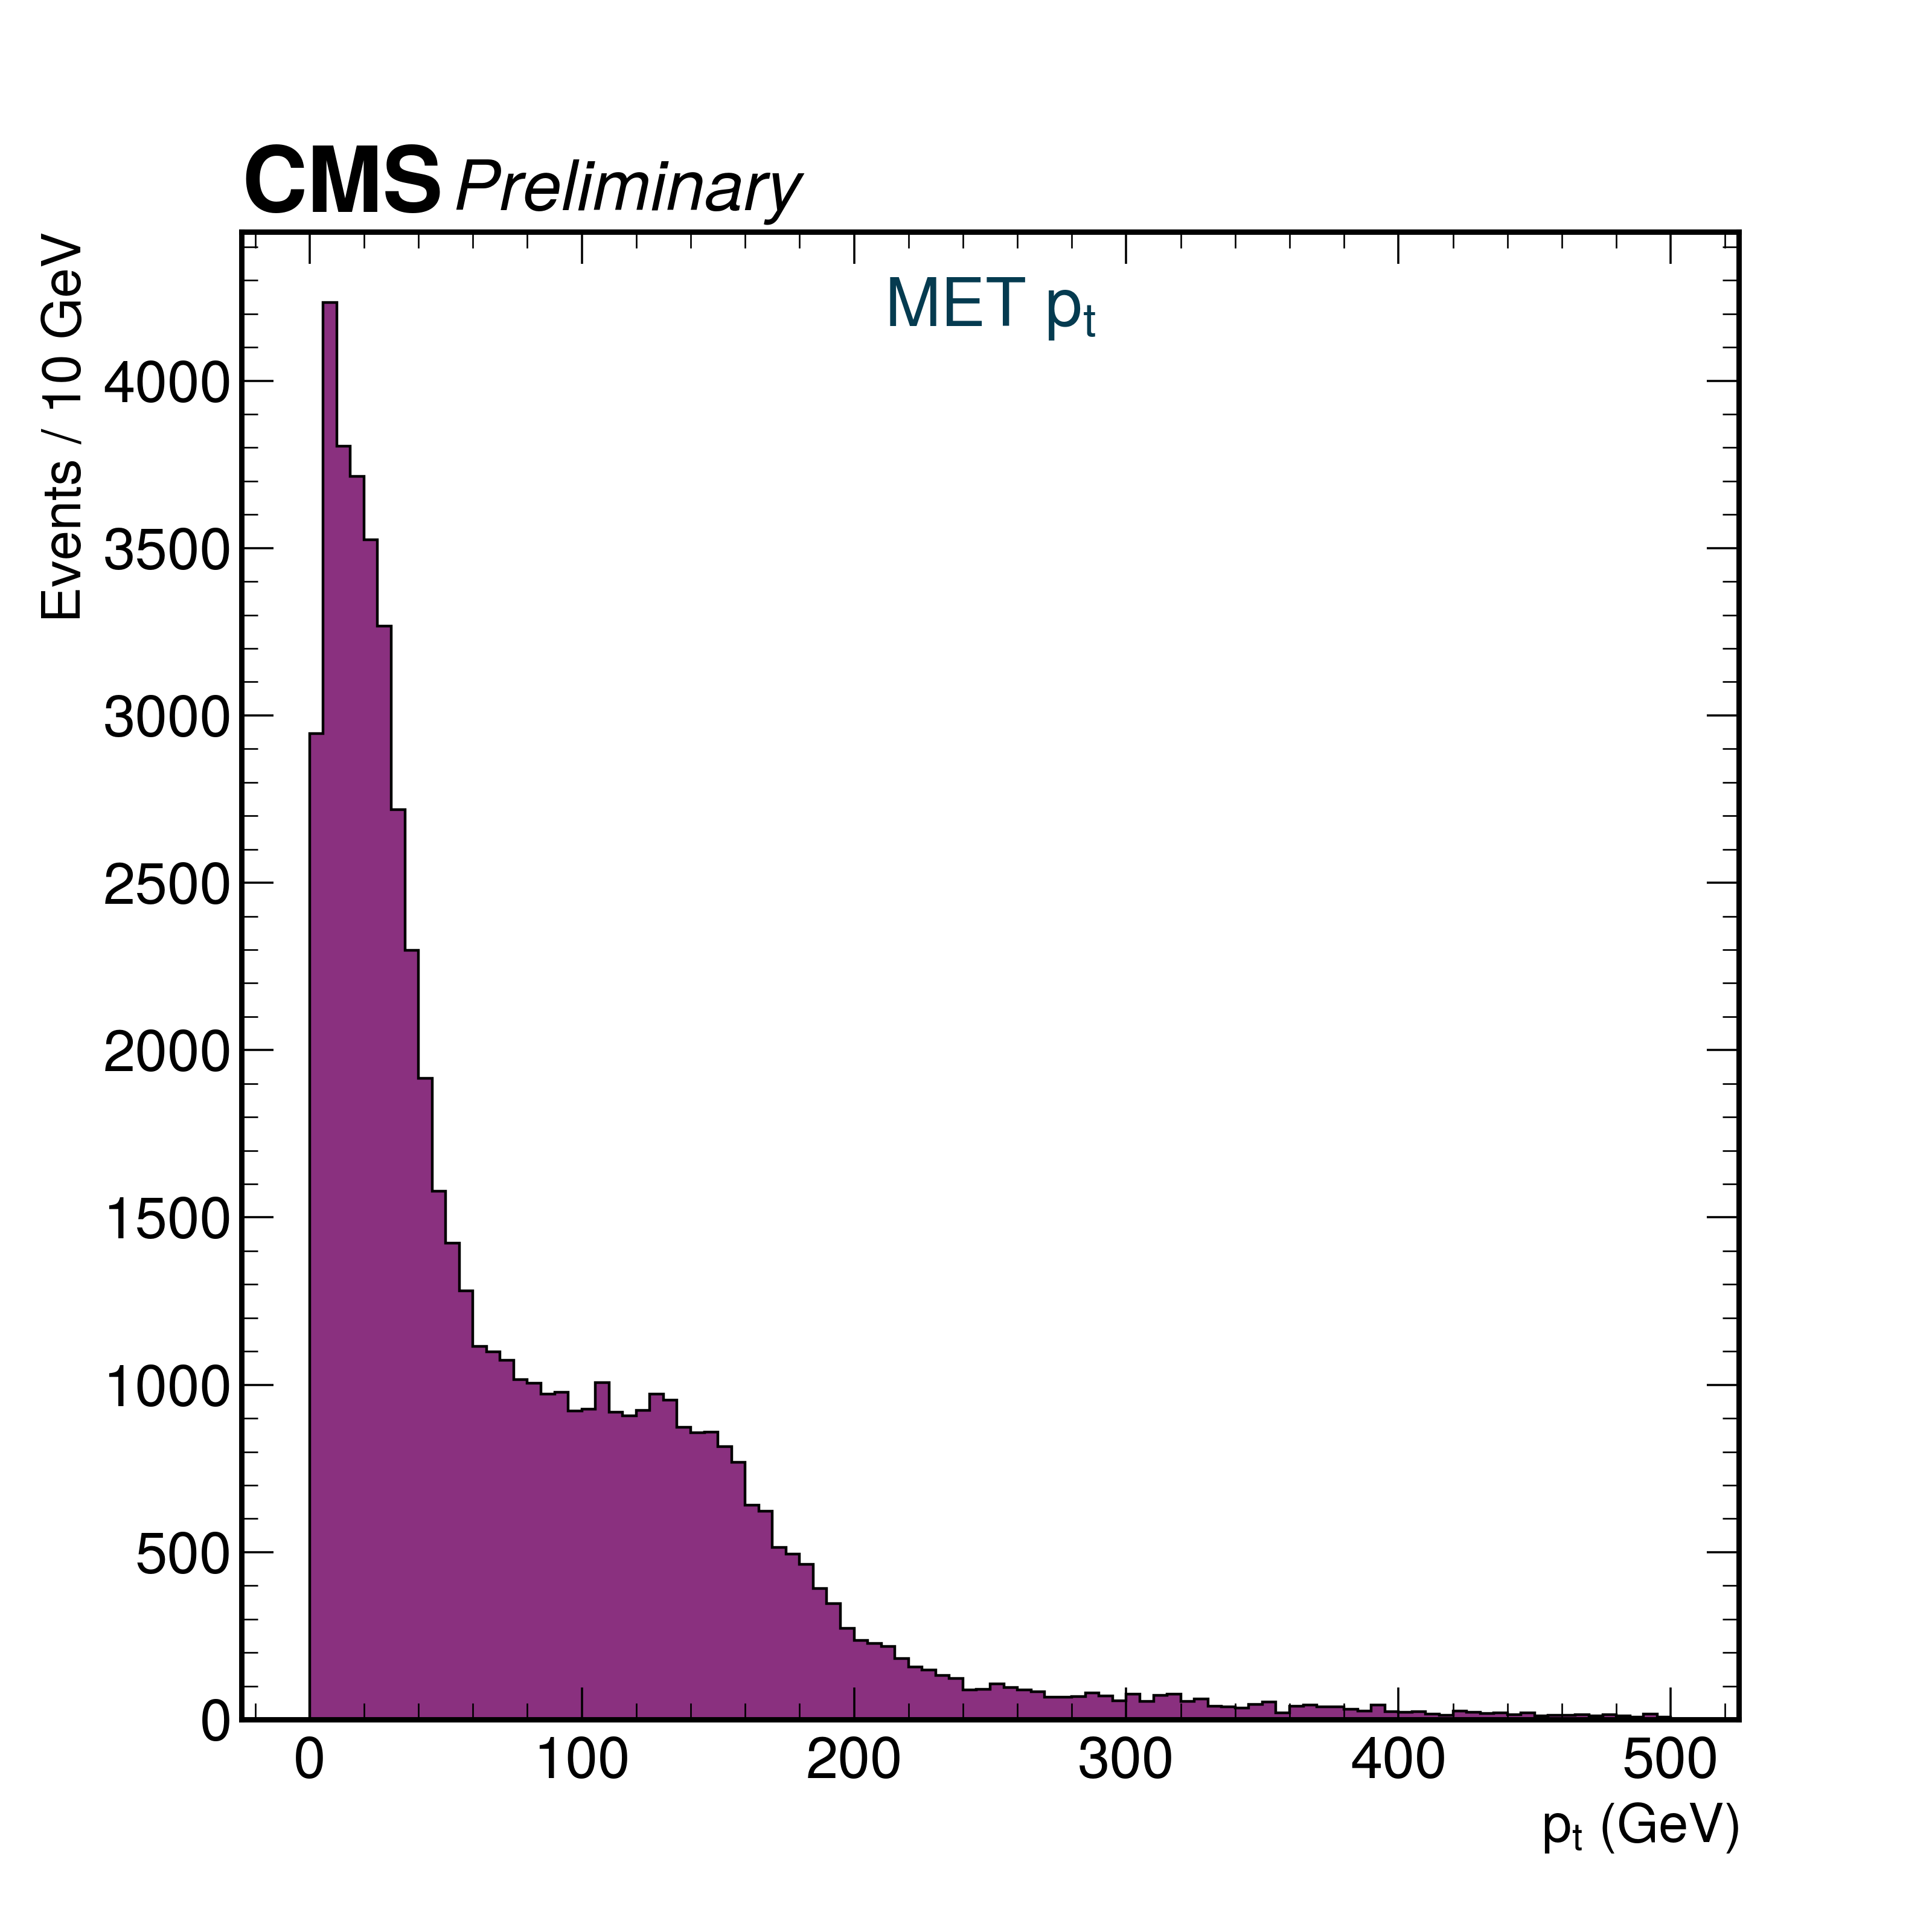
\includegraphics[width=1\textwidth]{../Archive/KinemPlots/METData.png }
    \label{METData} 
    \caption{MET $p_t$ for Data samples}
    \end{figure} 
    \column{0.38\textwidth} 
    \begin{itemize} 
    \raggedright 
    \small
    \item No filters or Trigger applied
    \item Looks similar to the Jet data
    \end{itemize}
    \end{columns} 
    \end{frame}

%%%%%%%%%%%%%%%%%%%%%%%%%%%%%%%%%%%%%%%%%%%%%%%%%%%%%%%%%%%%%%%%%%%%%%%%%%%%%%%%%%%%%%%%%%%%%%%%%%%%%%%%%%%%%%%%%%%%%%%%%%%%%%%%%%%%%%%%%%%%%%%%%%%%%%%%%%

\section[MET Filters ]{\small{Thu, $26^{th}$ October 2023 } \\ MET Filters / MET Flags}

  \begin{frame}[fragile]{MET $p_t$ : MET2018A} 
  \begin{columns}
  \column{0.58\textwidth} 
  \begin{figure} 
  \centering 
   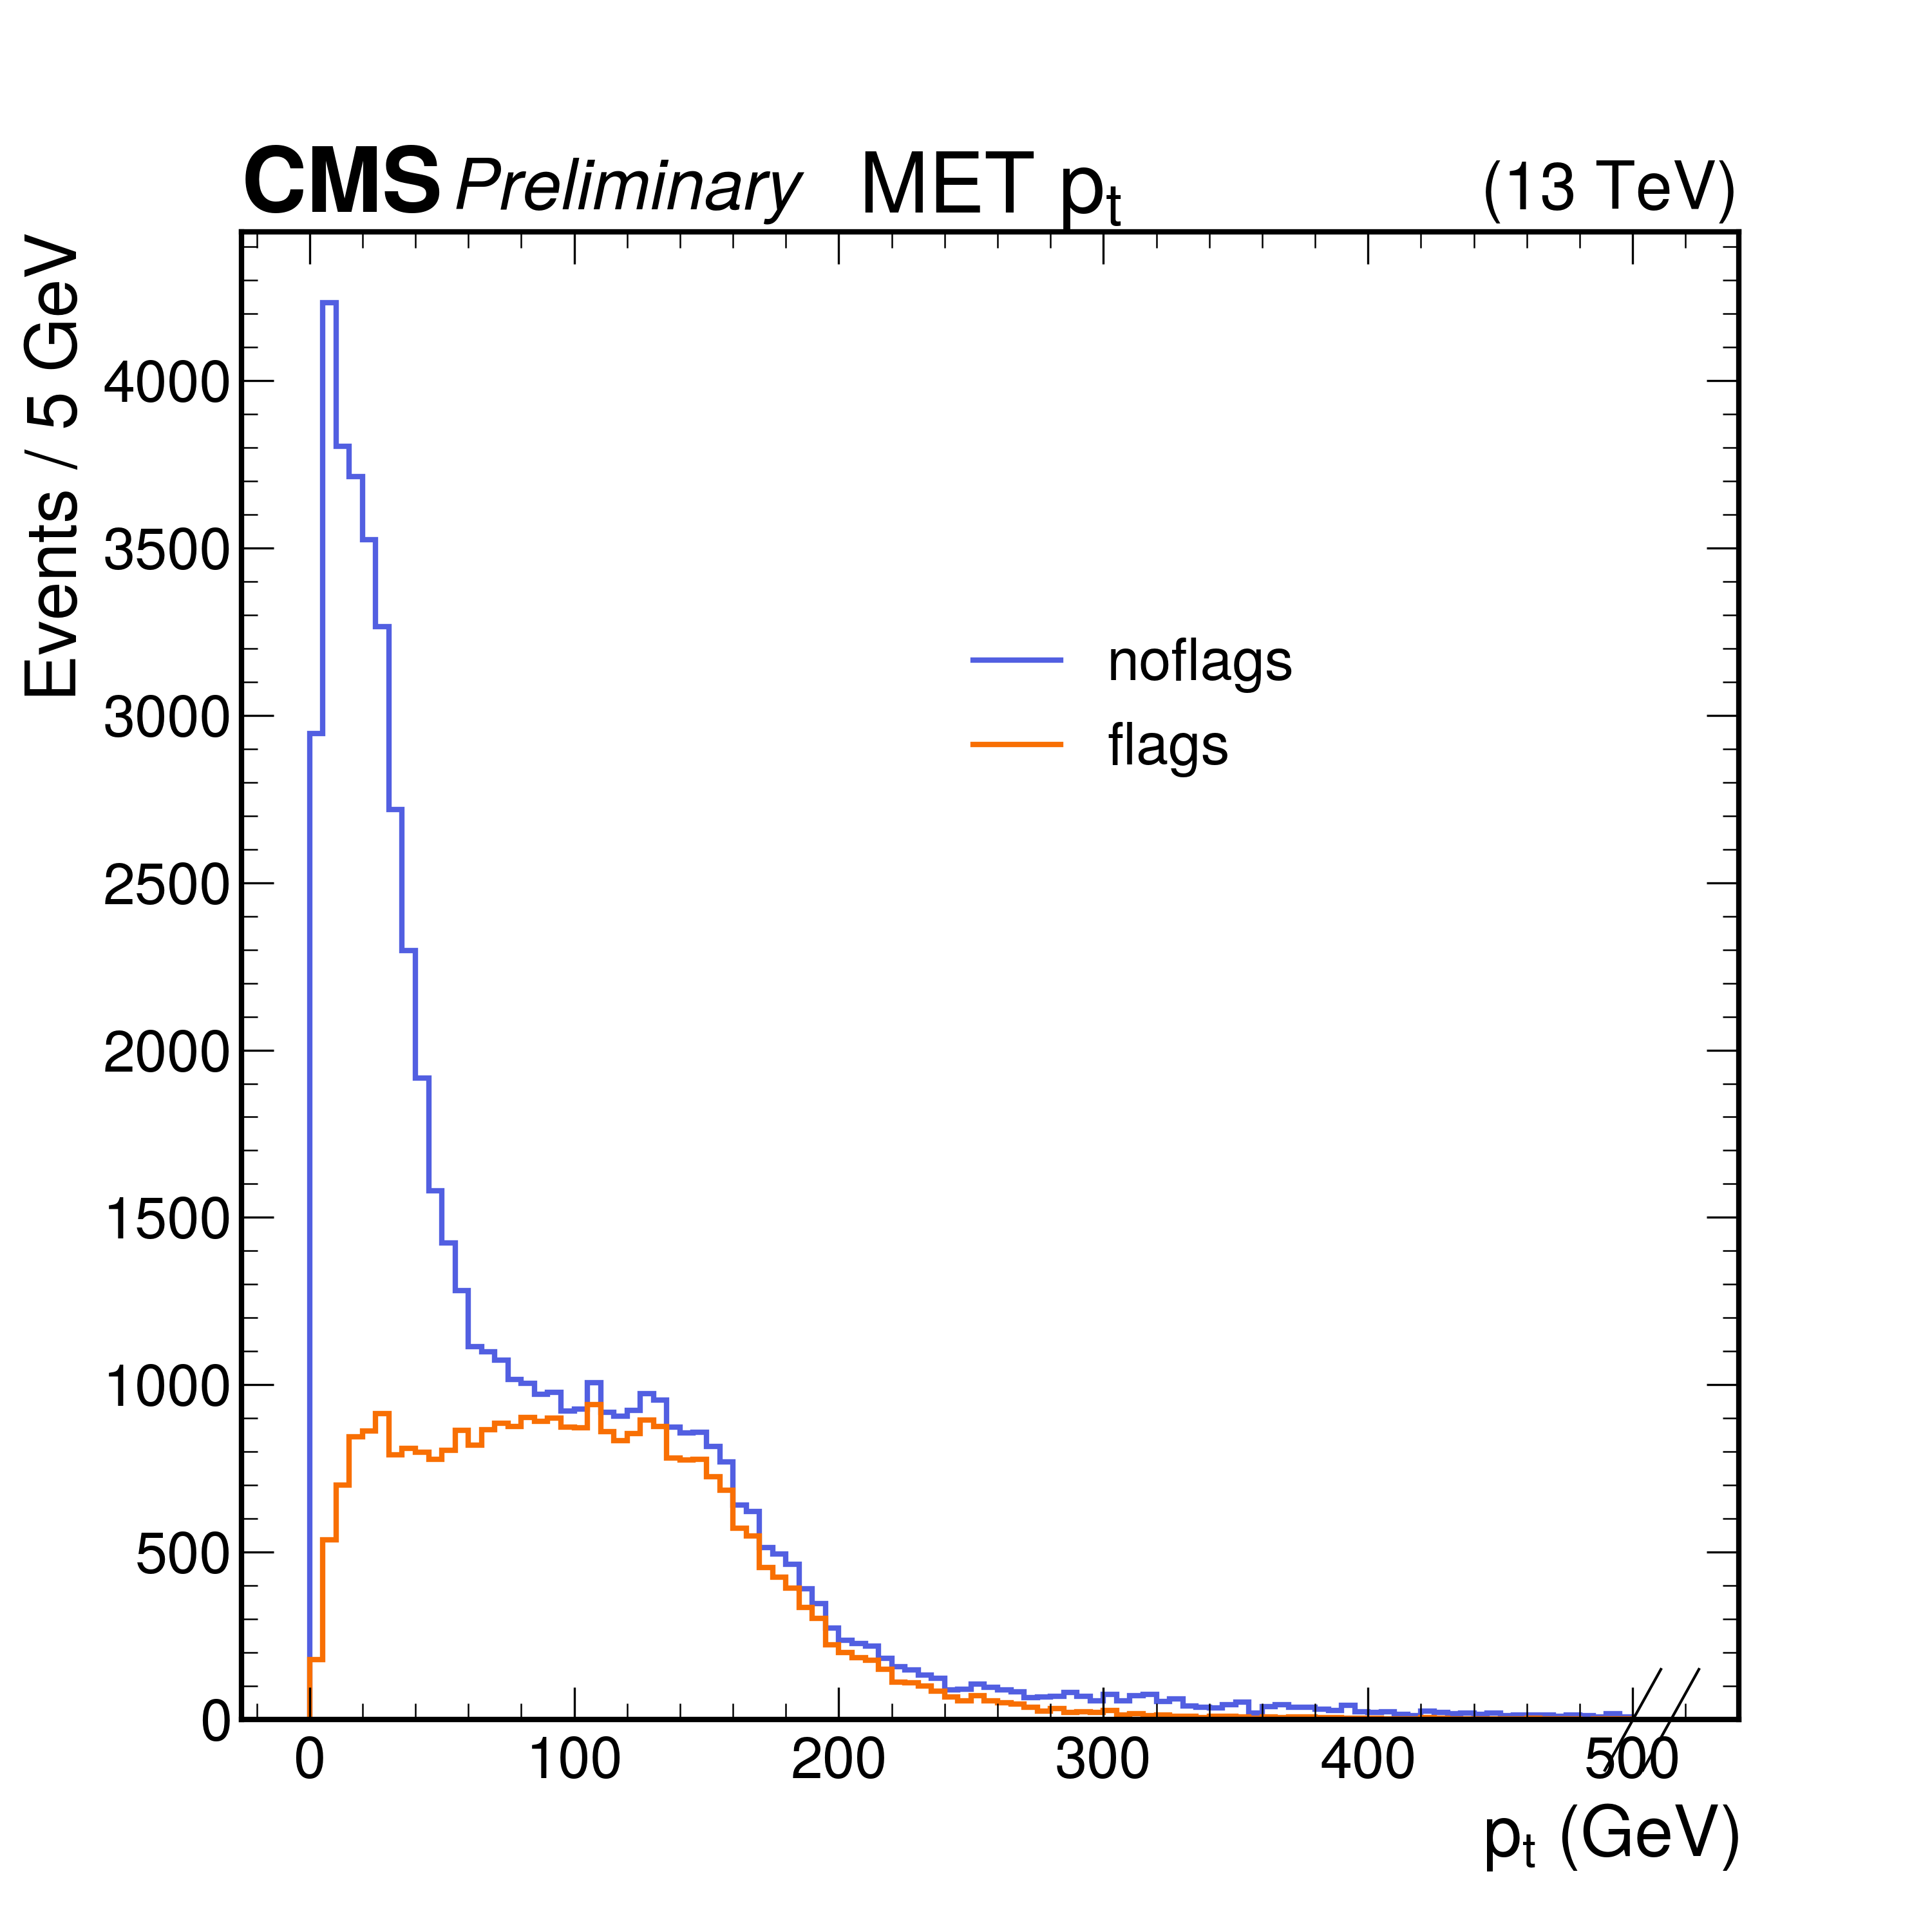
\includegraphics[width=1\textwidth]{../Archive/KinemPlots/DataptMETflags.png }
  \label{METDataflagpt} 
  \caption{MET $p_t$ for MET2018A}
  \end{figure} 
  \column{0.38\textwidth} 
  \begin{itemize} 
  \raggedright 
  \small
  \item Compared how the MET pt looks with and without MET triggers on Data
  \item .
  \end{itemize}
  \end{columns} 
  \end{frame}

  \begin{frame}[fragile]{MET $\phi$ : MET2018A} 
    \begin{columns}
    \column{0.58\textwidth} 
    \begin{figure} 
    \centering 
     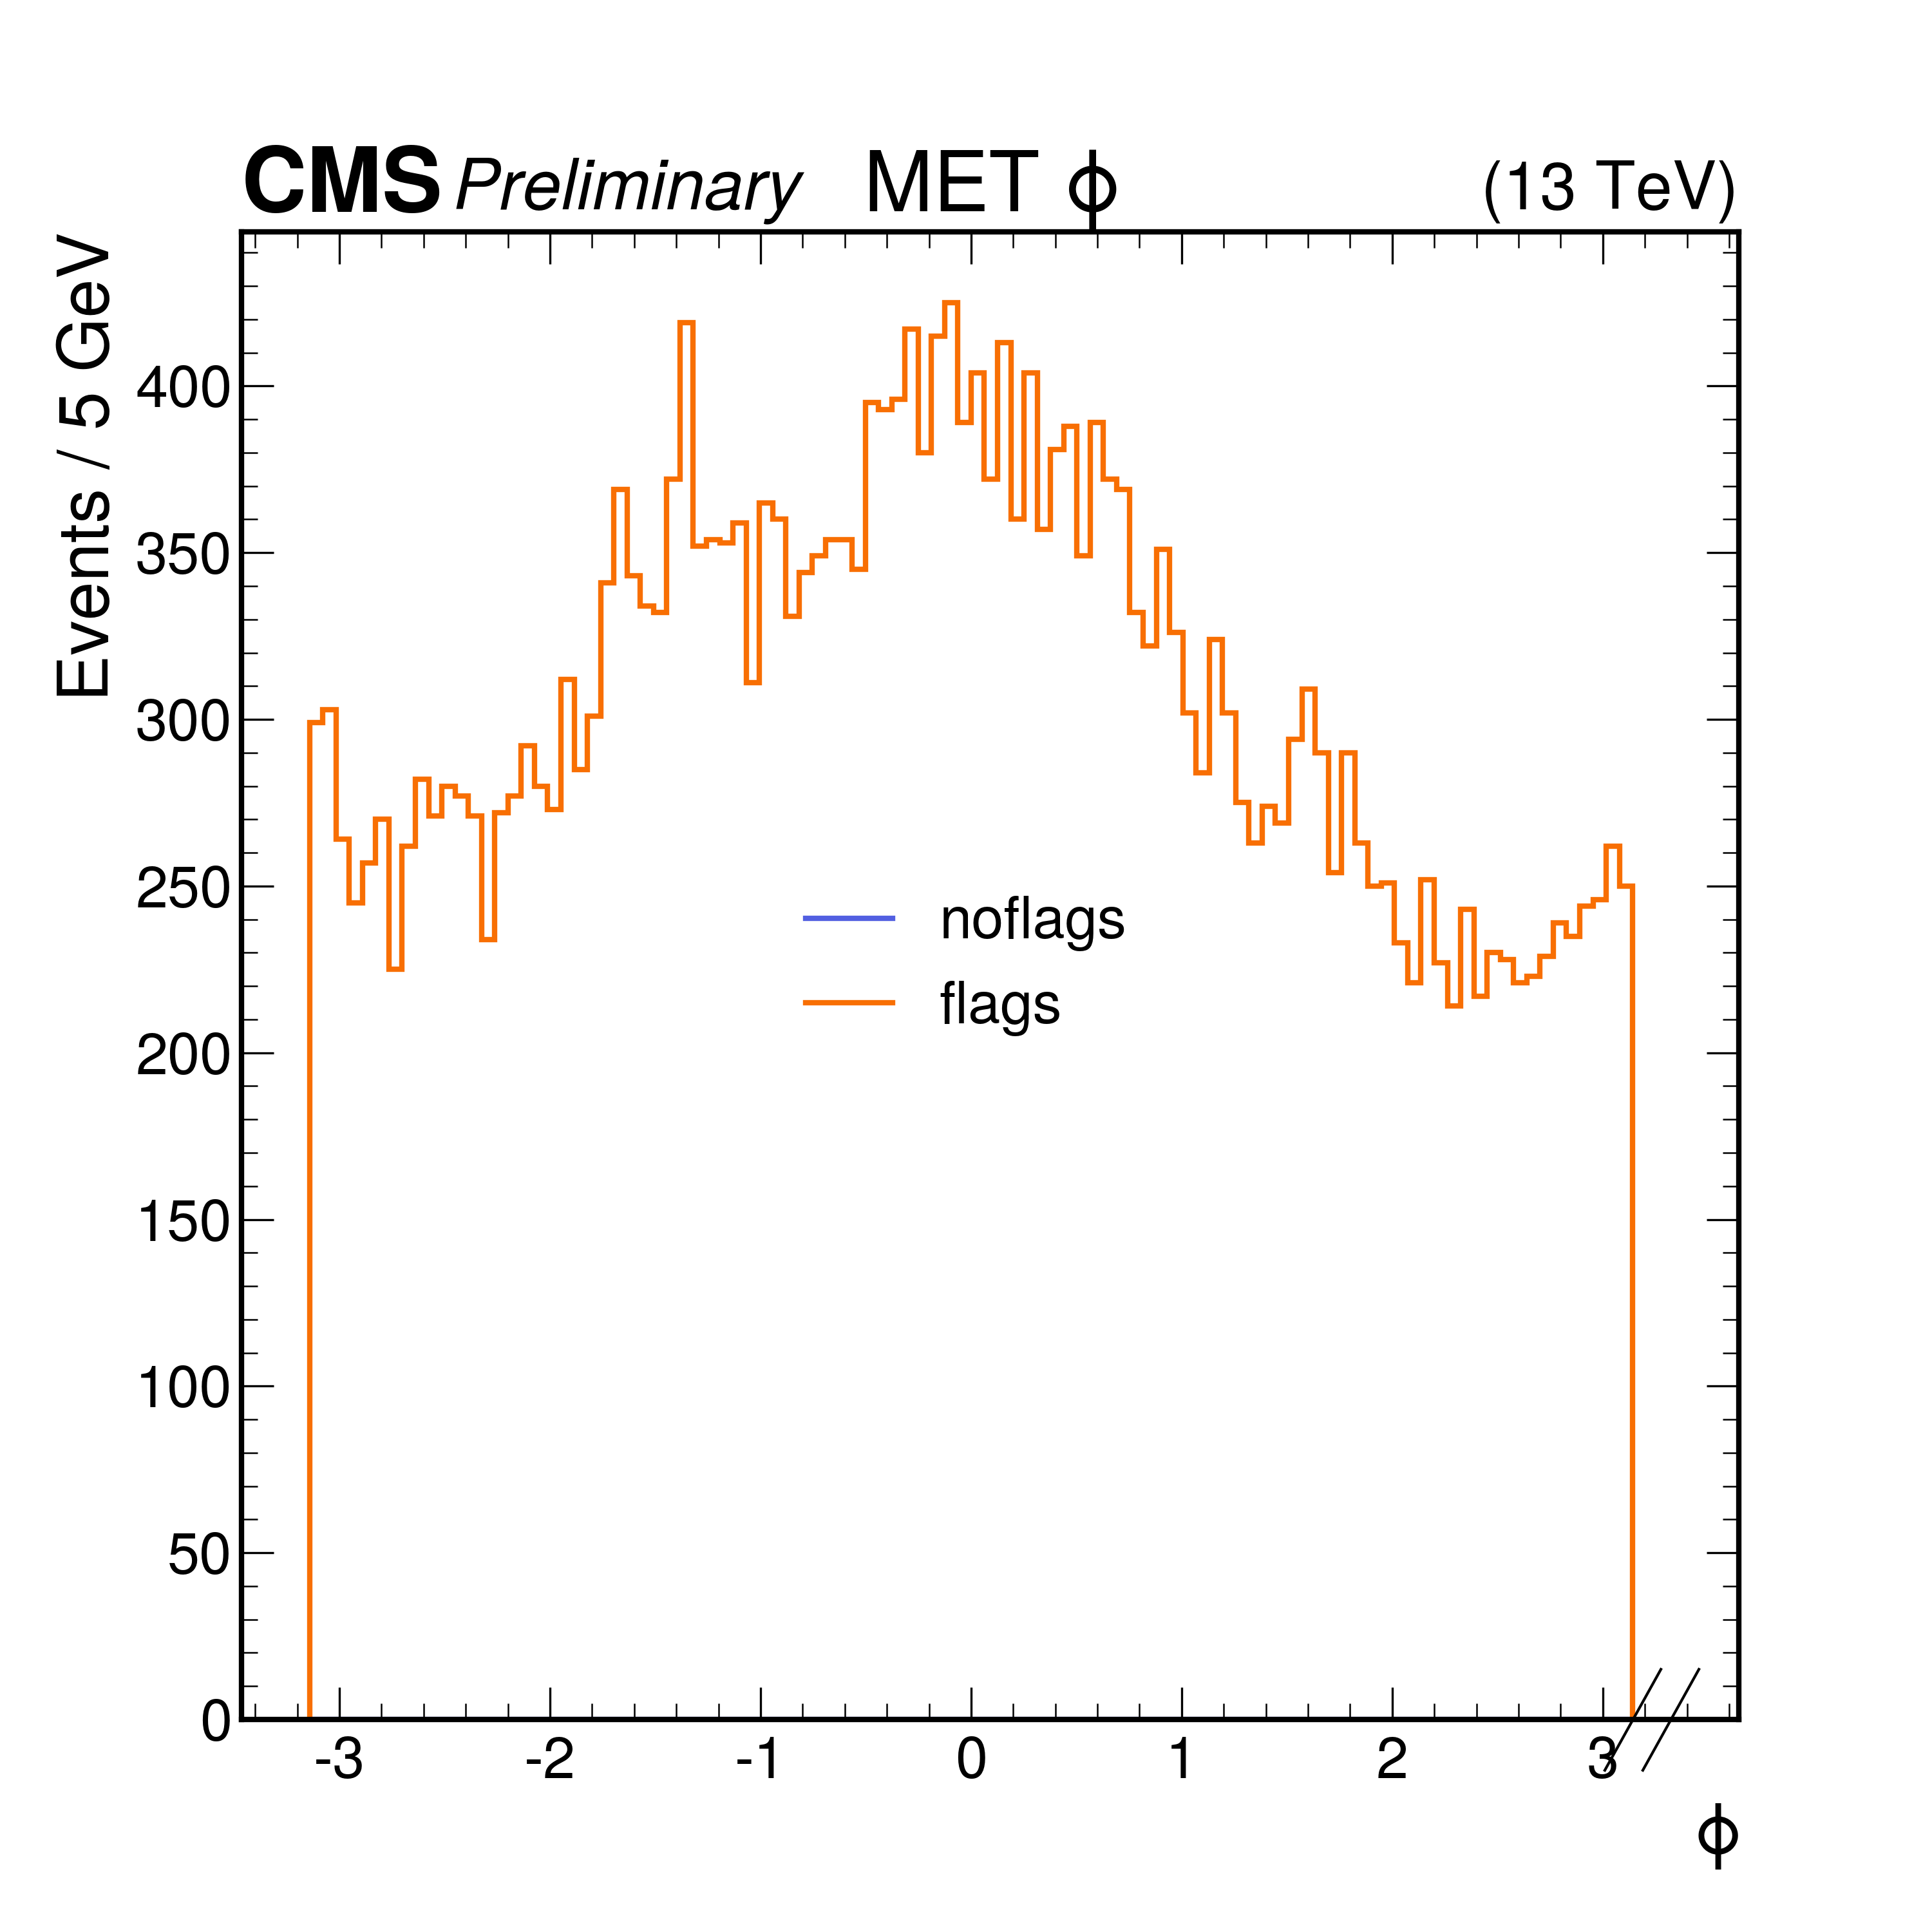
\includegraphics[width=1\textwidth]{../Archive/KinemPlots/DataphiMETflags.png }
    \label{METDataflagphi} 
    \caption{MET $\phi$ for MET2018A}
    \end{figure} 
    \column{0.38\textwidth} 
    \begin{itemize} 
    \raggedright 
    \small
    \item Compared how the MET $\phi$ looks with and without MET triggers
    \item .jf
    \end{itemize}
    \end{columns} 
    \end{frame}

  \begin{frame}[fragile]{MET $p_t$ : MonoHtobb\_ZpBaryonic} 
    \begin{columns}
    \column{0.58\textwidth} 
    \begin{figure} 
    \centering 
     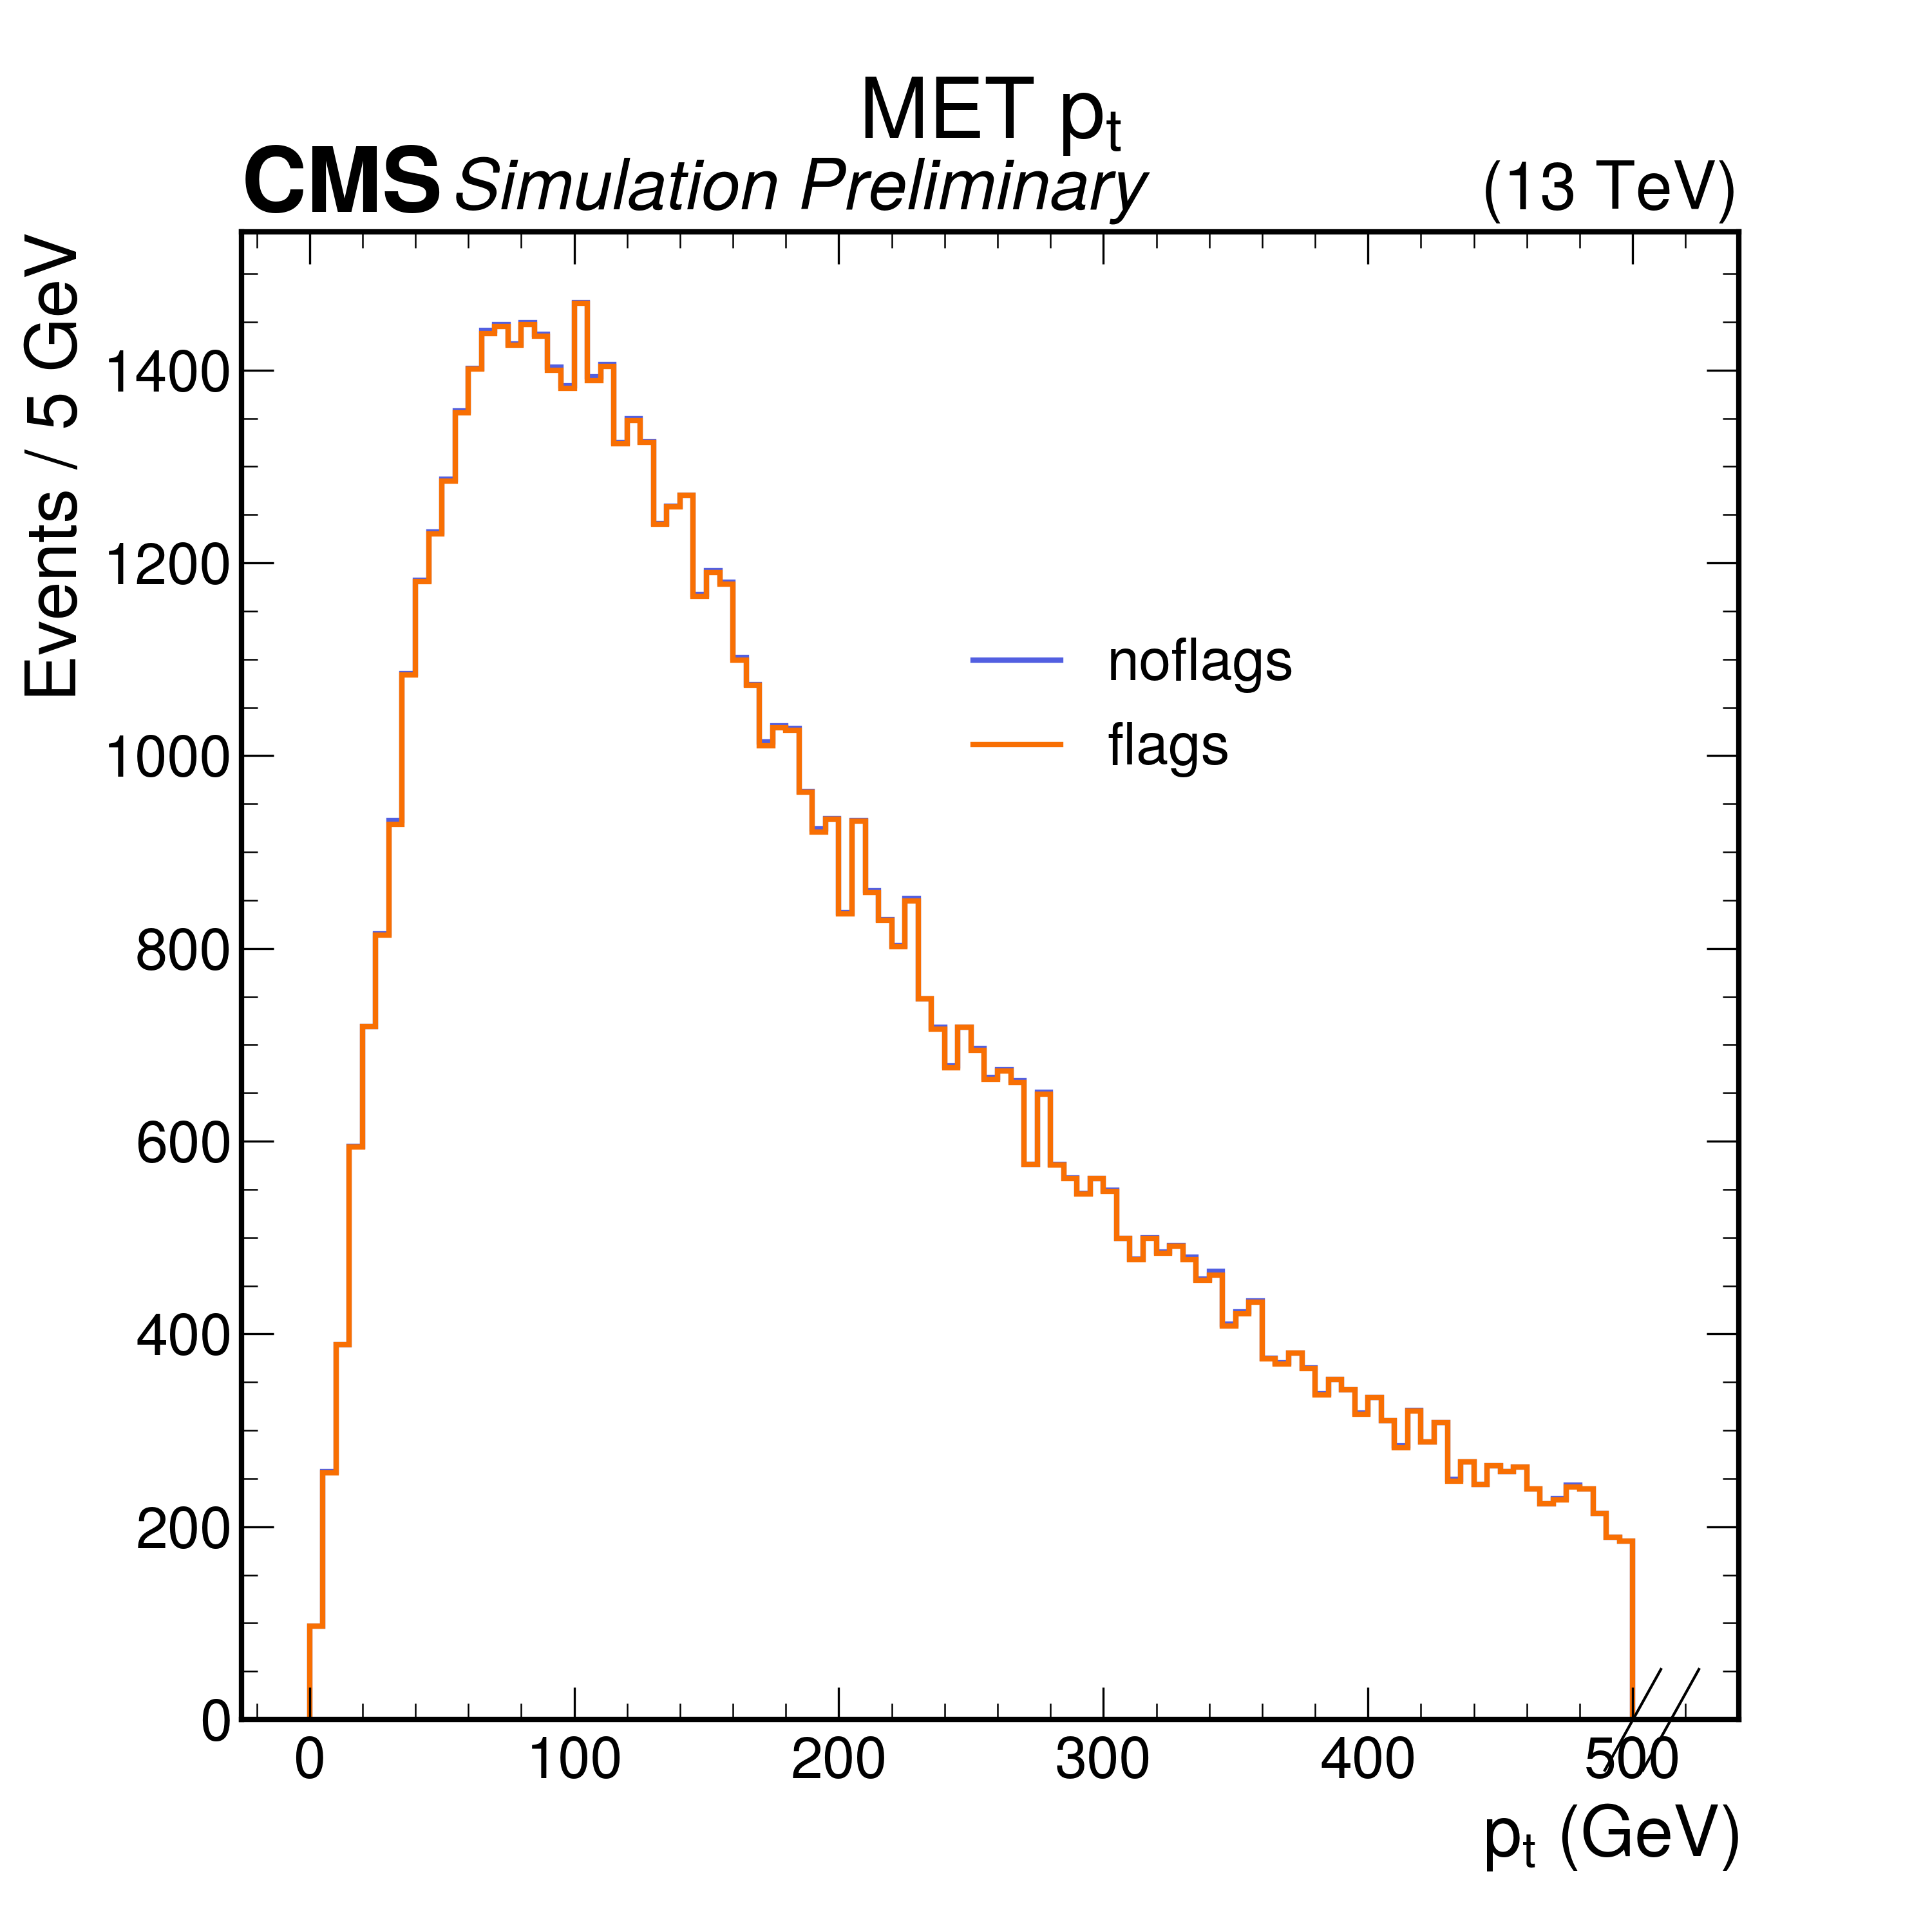
\includegraphics[width=1\textwidth]{../Archive/KinemPlots/MCptMETflags.png }
    \label{METMCflagpt} 
    \caption{MET $p_t$ for MonoHtobb\_ZpBaryonic}
    \end{figure} 
    \column{0.38\textwidth} 
    \begin{itemize} 
    \raggedright 
    \small
    \item Compared how the MET $p_t$ looks with and without MET triggers on Signal MC
    \item .jf
    \end{itemize}
    \end{columns} 
    \end{frame}

    \begin{frame}[fragile]{MET $\phi$ : MonoHTobb\_ZpBaryonic} 
      \begin{columns}
      \column{0.58\textwidth} 
      \begin{figure} 
      \centering 
       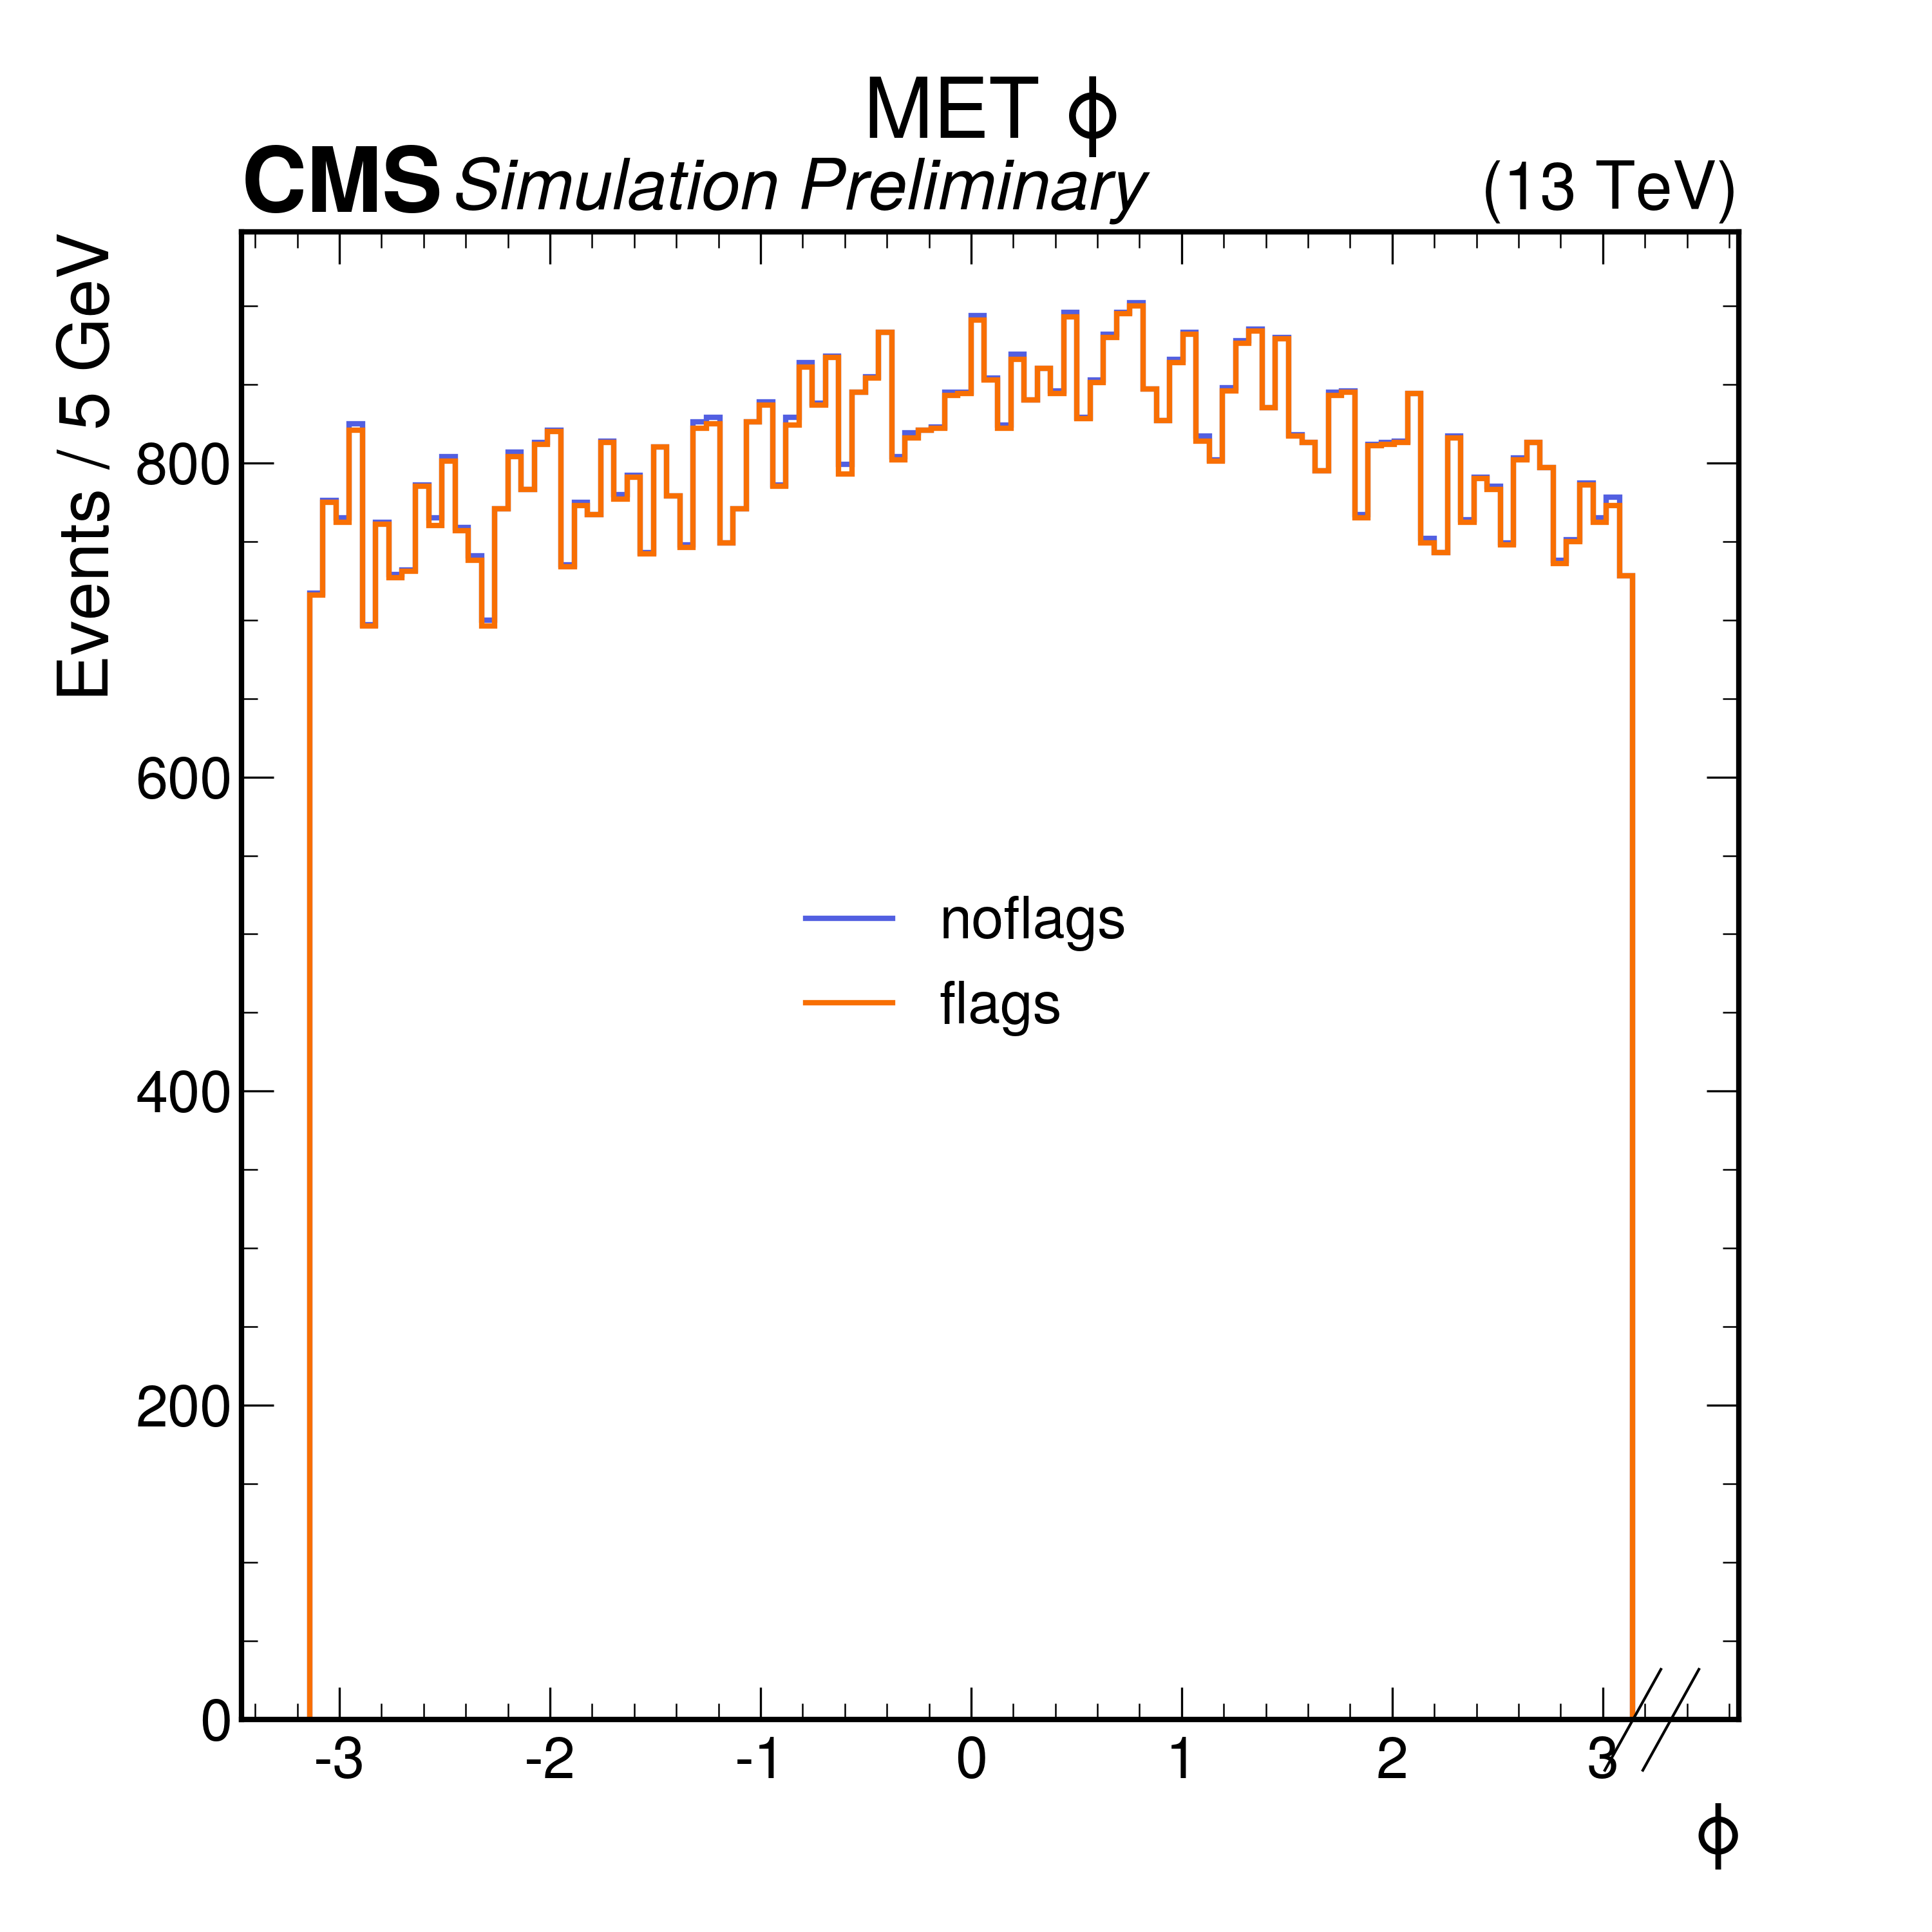
\includegraphics[width=1\textwidth]{../Archive/KinemPlots/MCphiMETflags.png }
      \label{METData} 
      \caption{MET $\phi$ for MC}
      \end{figure} 
      \column{0.38\textwidth} 
      \begin{itemize} 
      \raggedright 
      \small
      \item Compared how the MET $\phi$ looks with and without MET triggers on Signal MC
      \item .
      \end{itemize}
      \end{columns} 
      \end{frame}

%%%%%%%%%%%%%%%%%%%%%%%%%%%%%%%%%%%%%%%%%%%%%%%%%%%%%%%%%%%%%%%%%%%%%%%%%%%%%%%%%%%%%%%%%%%%%%%%%%%%%%%%%%%%%%%%%%%%%%%%%%%%%%%%%%%%%%%%%%%%%%%%%%%%%%%%%%

% \section[Backgrounds ]{\small{Thu, $26^{th}$ October 2023 } \\ Backgrounds}

%%%%%%%%%%%%%%%%%%%%%%%%%%%%%%%%%%%%%%%%%%%%%%%%%%%%%%%%%%%%%%%%%%%%%%%%%%%%%%%%%%%%%%%%%%%%%%%%%%%%%%%%%%%%%%%%%%%%%%%%%%%%%%%%%%%%%%%%%%%%%%%%%%%%%%%%%%

\section[Contribution of various backgrounds]{\small{\today} \\ Tue, $2^{nd}$ January 2024 }

%%%%%%%%%%%%%%%%%%%%%%%%%%%%%%%%%%%%%%%%%%%%%%%%%%%%%%%%%%%%%%%%%%%%%%%%%%%%%%%%%%%%%%%%%%%%%%%%%%%%%%%%%%%%%%%%%%%%%%%%%%%%%%%%%%%%%%%%%%%%%%%%%%%%%%%%%%

     \begin{frame}[fragile]{Contribution of various backgrounds: Resolved b$ \bar{b} $ bar in 2018}
      \begin{columns}
        \column{0.58\textwidth}
        \begin{figure}
          \centering
          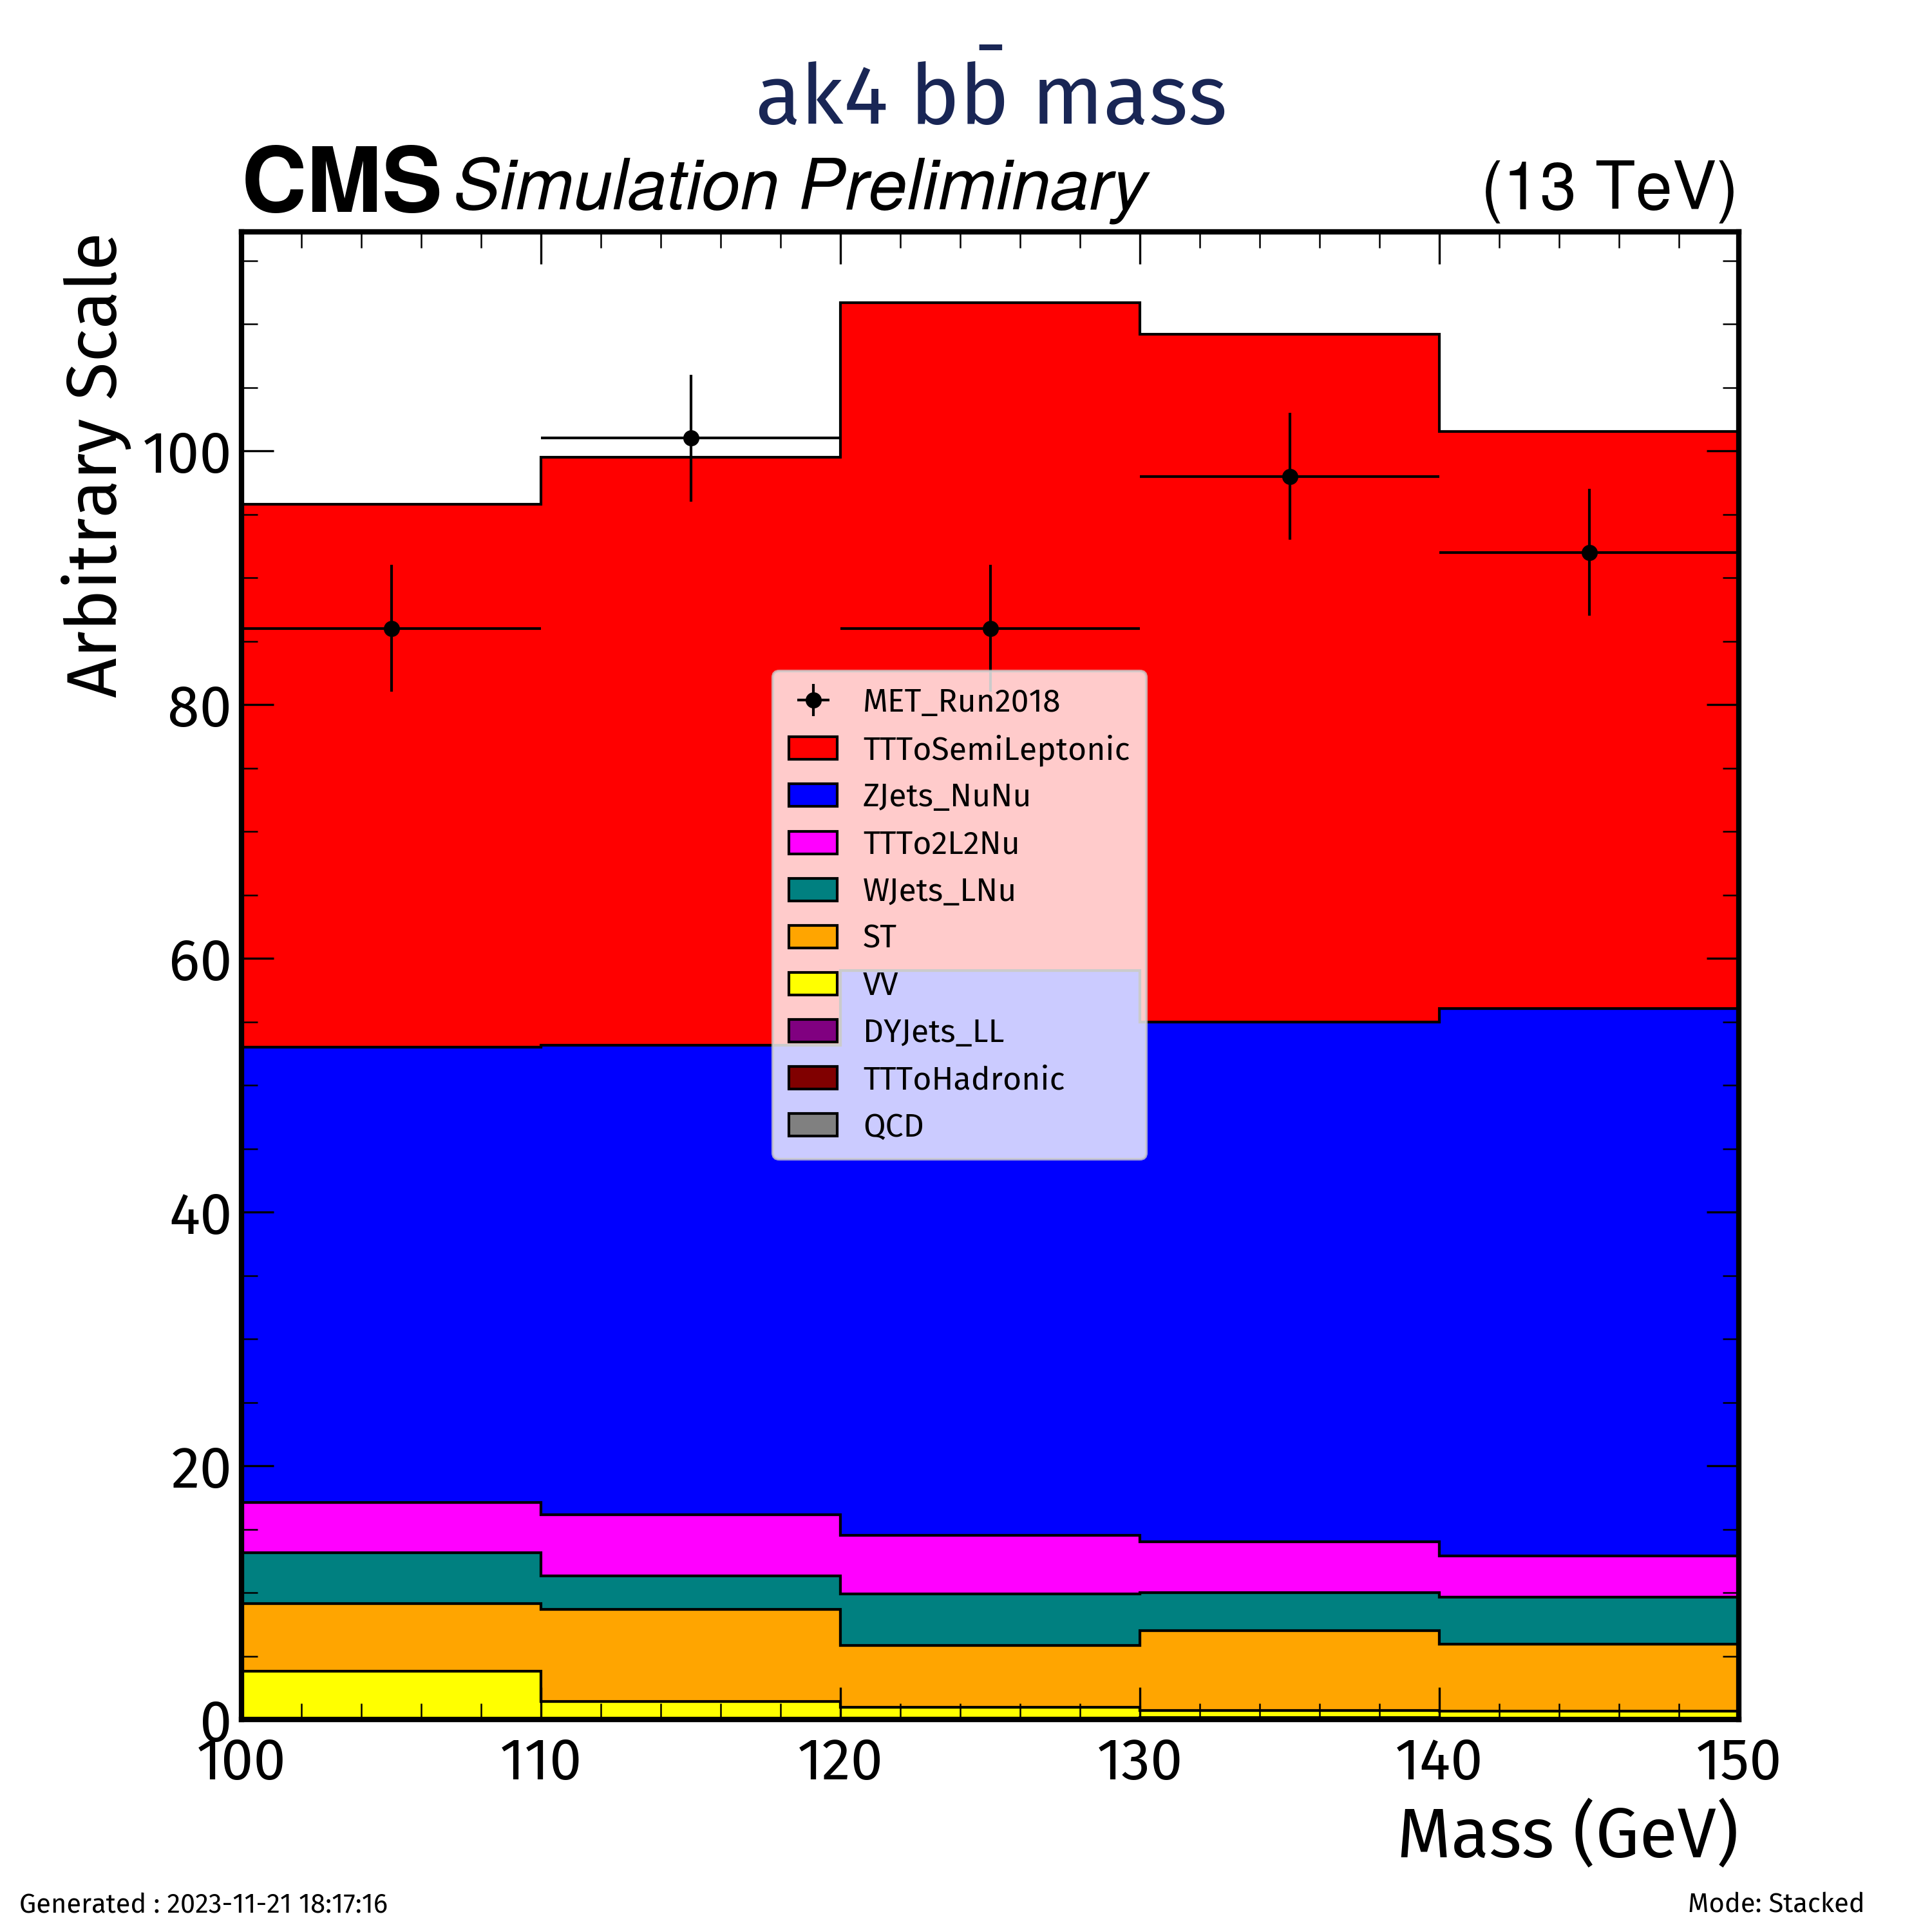
\includegraphics[width=1\textwidth]{../Backgrounds/plots/SR_Resolved_Backgrounds_dijet_mass_Combined.png}
          \label{contribution}
          \caption{Simulated contribution of various backgrounds to the signal in the resolved b$ \bar{b} $ bar case for 2018}
        \end{figure}
        \column{0.38\textwidth}
        Selections Applied: 
        Event Selections:
        \begin{itemize}
          \raggedright 
          \tiny
          \item {MET > 200 GeV}
          \item {no leptons}
          \item {no photons}
        \end{itemize}
        Object Selections:
        \begin{itemize}
          \raggedright 
          \tiny
          \item {jet $p_t > 30 $ GeV}
          \item {jet $| \eta | < 2.5 $}
          \item {$\Delta \phi (Jet, \ MET)$}
          \item {at least 2 tight bjets (algorithm:DeepFlavB)}
          \item {leading bjet $p_t > 50 $ GeV}
          \item {subleading bjet $p_t > 30 $ GeV}
          \item {atmost 2 additional jets}
          \item {dijet = leading bjet + subleading bjet}
          \item {dijet mass between (100 GeV,150 GeV)}
          \item {dijet $p_t > 100 $ GeV}
        \end{itemize}
      \end{columns}
    \end{frame}

%%%%%%%%%%%%%%%%%%%%%%%%%%%%%%%%%%%%%%%%%%%%%%%%%%%%%%%%%%%%%%%%%%%%%%%%%%%%%%%%%%%%%%%%%%%%%%%%%%%%%%%%%%%%%%%%%%%%%%%%%%%%%%%%%%%%%%%%%%%%%%%%%%%%%%%%%%


%%%%%%%%%%%%%%%%%%%%%%%%%%%%%%%%%%%%%%%%%%%%%%%%%%%%%%%%%%%%%%%%%%%%%%%%%%%%%%%%%%%%%%%%%%%%%%%%%%%%%%%%%%%%%%%%%%%%%%%%%%%%%%%%%%%%%%%%%%%%%%%%%%%%%%%%%%

% \section[Section label]{\small{\today} \\ Thu, $5^{th}$ October 2023  }

% %%%%%%%%%%%%%%%%%%%%%%%%%%%%%%%%%%%%%%%%%%%%%%%%%%%%%%%%%%%%%%%%%%%%%%%%%%%%%%%%%%%%%%%%%%%%%%%%%%%%%%%%%%%%%%%%%%%%%%%%%%%%%%%%%%%%%%%%%%%%%%%%%%%%%%%%%%

%      \begin{frame}[fragile]{Frame title}
%       \begin{columns}
%         \column{0.58\textwidth}
%         \begin{figure}
%           \centering
%           
\includegraphics[width=1\textwidth]{uoh_logo.png}
%           \label{plot label}
%           \caption{Your caption}
%         \end{figure}
%         \column{0.38\textwidth}
%         \begin{itemize}
%           \raggedright 
%           \small
%           \item {point 1}
%           \item {point 2}
%         \end{itemize}
%       \end{columns}
%     \end{frame}

% %%%%%%%%%%%%%%%%%%%%%%%%%%%%%%%%%%%%%%%%%%%%%%%%%%%%%%%%%%%%%%%%%%%%%%%%%%%%%%%%%%%%%%%%%%%%%%%%%%%%%%%%%%%%%%%%%%%%%%%%%%%%%%%%%%%%%%%%%%%%%%%%%%%%%%%%%%

\appendix

% \begin{frame}[fragile]{Backup slides}

% \end{frame}

\begin{frame}[allowframebreaks]{References}

  \bibliography{references}
  \bibliographystyle{abbrv}

\end{frame}

\end{document}
